% =====================================================================
% Structure-Aware Row Scaling for Block-Structured Mixed-Integer Programs
% International Journal for Numerical Methods in Engineering (Wiley) -- NJD v5.
%
% COMPILE WITH XeLaTeX on TeX Live 2022 (the WileyNJDv5 class requires XeLaTeX;
% the template states TeX Live 2023 is unsupported). Sequence:
%   xelatex main ; bibtex main ; xelatex main ; xelatex main
% AMA = the journal reference style; Times1COL = single-column review layout.
% =====================================================================
\documentclass[AMA,Times1COL]{WileyNJDv5}

% --- Packages NOT already provided by WileyNJDv5 (which loads amsmath, amsthm,
%     amssymb, graphicx, hyperref, booktabs, multirow, threeparttable, float,
%     subfig, xcolor, url, ...). Only additive packages are loaded here. ---
\usepackage{mathtools}
\usepackage{bm}
\usepackage{threeparttable}
\usepackage{placeins}    % \FloatBarrier (class does not load it)
\usepackage{subcaption}  % subfig not active in this class mode; caption is loaded
\usepackage{siunitx}
\sisetup{
  detect-weight=true,
  detect-family=true,
  detect-mode=text,
  mode=text,
  group-digits=integer,
  group-minimum-digits=4,
  group-separator={,},
  table-number-alignment=center,
}
\usepackage{algorithm}
\usepackage{algpseudocode}
% orcidlink removed: fragile inside NJD \maketitle; ORCID given as text in \corres
\usepackage{lineno}                       % continuous line numbers for review
\usepackage{tikz}                          % conceptual overview figure (Fig. 1)
\usetikzlibrary{arrows.meta,positioning,calc}
\usepackage[nameinlink,noabbrev]{cleveref} % after the class-loaded hyperref

% Open in single-page (continuous) layout. The title page is an odd, right-hand page;
% in a two-page/"book" viewer the reader sees a blank sheet to its left, which reads as a
% phantom blank first page. This hint makes compliant viewers default to one page wide, so
% no facing blank appears. It only sets the default view; it changes no content.
\hypersetup{pdfpagelayout=OneColumn}

% --- Macros (theorem environments and caption styling are provided by the class) ---
\newcommand{\R}{\mathbb{R}}
\newcommand{\Z}{\mathbb{Z}}
\newcommand{\nnz}{\operatorname{nnz}}
\newcommand{\diag}{\operatorname{diag}}
\newcommand{\cond}{\operatorname{cond}}
\newcommand{\argmin}{\operatorname*{arg\,min}}
\newcommand{\norm}[1]{\left\lVert #1 \right\rVert}
\newcommand{\abs}[1]{\left\lvert #1 \right\rvert}
\newcommand{\methodBase}{Base}
\newcommand{\methodAug}{SA-Aug}
\newcommand{\methodMat}{SA-Mat}
\newcommand{\methodRuiz}{Ruiz}
\newcommand{\methodRuizCols}{Ruiz+Cols}
\newcommand{\sgm}{\ensuremath{\operatorname{sgm}}}
\newcommand{\PARten}{\ensuremath{\operatorname{PAR10}}}
\newcommand{\PI}{\ensuremath{\operatorname{PI}}}
\newcommand{\Work}{\texttt{Work}}

% Figure helpers. Figures are external vector PDFs in figs/. The two-panel helper
% uses the subfigure environment from subcaption (loaded above), not the class's subfig.
\newcommand{\singleplotheight}{.42\textheight}
\newcommand{\pairedplotheight}{.30\textheight}
\newcommand{\safefigure}[2]{\includegraphics[width=#2,keepaspectratio]{#1}}
\newcommand{\plotfigure}[4]{%
  \begin{figure*}[!tbp]
  \centering
  \includegraphics[width=#2,height=\singleplotheight,keepaspectratio]{#1}
  \caption{#3}\label{#4}
  \end{figure*}%
}
\newcommand{\plotfiguretrim}[5][3pt 3pt 3pt 3pt]{%
  \begin{figure*}[!tbp]
  \centering
  \includegraphics[width=#3,height=\singleplotheight,trim=#1,clip,keepaspectratio]{#2}
  \caption{#4}\label{#5}
  \end{figure*}%
}
\newcommand{\twoplotfigure}[8]{%
  \begin{figure*}[!tbp]
  \centering
  \begin{subfigure}[t]{0.485\textwidth}\centering
    \includegraphics[width=\linewidth,height=\pairedplotheight,clip,keepaspectratio]{#1}
    \caption{#2}\label{#3}
  \end{subfigure}\hfill
  \begin{subfigure}[t]{0.485\textwidth}\centering
    \includegraphics[width=\linewidth,height=\pairedplotheight,clip,keepaspectratio]{#4}
    \caption{#5}\label{#6}
  \end{subfigure}
  \caption{#7}\label{#8}
  \end{figure*}%
}

\graphicspath{{figs/}}

% --- Front matter (NJD v5) ---
\articletype{Research Article}
\received{}
\revised{}
\accepted{}
% Pin the running folio so the title page is numbered 1 (the class otherwise leaves
% the start-page placeholder unset and prints "0" on the title page, which reads as a
% missing/blank first page); the journal overrides this at production.
\startpage{1}

\begin{document}

\title{Structure-Aware Row Scaling for Block-Structured Mixed-Integer Programs}

\author[1]{Mathias Rodr\'iguez Castro}

\authormark{Rodr\'iguez Castro}
\titlemark{Structure-Aware Row Scaling for Block-Structured Mixed-Integer Programs}

\address[1]{\orgdiv{Facultad de Ingenier\'ia}, \orgname{Universidad de la Rep\'ublica}, \orgaddress{\state{Montevideo}, \country{Uruguay}}}

\corres{Mathias Rodr\'iguez Castro, Facultad de Ingenier\'ia, Universidad de la Rep\'ublica, Montevideo, Uruguay. \email{mathiasr@fing.edu.uy} (ORCID: 0009-0002-7235-7677)}

\abstract[Abstract]{%
Generated mixed-integer programs (MIPs) are usually exported to solvers as flat coefficient matrices, yet the generator that builds them knows which constraints are local to physical components, which variables those components own, and which rows couple components through system-wide balances. We ask whether this pre-export metadata can drive positive row scaling without changing the program. We propose a structure-aware row-scaling framework for block-structured MIPs: complete constraints, including right-hand sides, are multiplied by strictly positive factors, so the feasible set, objective, and integer restrictions are preserved exactly. The contribution is not row scaling itself, but using generator metadata to order it---local rows first, then representative block scales, then coupling rows relative to the blocks they connect---which an idealized conditioning analysis shows separates local from coupling imbalance. We evaluate the method on a hydrothermal dispatch platform emitting modular MIPs, treated as a generated block-structured testbed rather than a hydro-specific application; the only metadata required are row roles, block ownership, and coupling incidence. Across three instance classes, two solvers, and two optimality tolerances, positive row scaling is algebraically exact, structure-aware scaling robustly improves solver-facing numerical diagnostics, and runtime drops under Gurobi but not robustly under CPLEX. A role-blind control, however, locates the runtime effect in complete per-row scaling rather than in the metadata: the same kernel applied to every row matches the structure-aware rule on the simpler class and beats it on the coupled one. The metadata's value is thus in the numerical representation---the rule that best conditions the matrix is not the one that solves fastest---so the method is best read as a structure-aware numerical preprocessing layer, not a solver-independent acceleration theorem.
}

\keywords{Numerical scaling, mixed-integer programming, generated formulations, block-structured optimization, engineering optimization, hydrothermal dispatch}

\maketitle

% Review builds carry continuous line numbers; set \reviewversionfalse for production.
\newif\ifreviewversion
\reviewversiontrue
\ifreviewversion\linenumbers\fi

\section*{Practitioner Points}
\begin{itemize}
  \item Model generators know each row's role, block ownership, and coupling incidence---metadata
  a flat export discards but that can drive numerical preprocessing.
  \item Positive, structure-keyed row factors applied in a local--block--coupling order improve
  the solver-facing representation without changing the MIP.
  \item The runtime lever, however, is \emph{complete} per-row normalization, not the row-role
  metadata: a rule that scales only the rows it recognizes by role can miss the worst-scaled
  rows, so a practical layer should cover every row rather than rely on role sophistication.
  \item The runtime benefit is also solver-dependent---present under Gurobi, absent under
  CPLEX---so scaling gains should be validated per solver, not assumed.
\end{itemize}


% -------------------------------------------------------------------------
\section{Introduction}
\label{sec:introduction}
% -------------------------------------------------------------------------

A model generator and a solver see different representations of the same optimization problem. The generator builds the model from components: hydro plants, thermal units, market rules, resource limits, demand balances, and discrete operating decisions. While doing so, it knows which rows are local to one component, which variables that component owns, and which constraints link several components. The solver receives the exported version: rows, columns, coefficients, bounds, and tolerances. In that exported matrix, much of the generator's structural knowledge has disappeared.

This loss matters because numerical representation affects computation. Two formulations
can describe the same feasible set and objective, yet lead a solver through different
presolve reductions, relaxation bases, cuts, incumbent searches, branching decisions, and
feasibility checks. Generic scaling routines can inspect coefficient magnitudes after
export. They usually cannot tell whether a row is a local turbine restriction, a thermal
limit, or a system-wide balance. The generator can make that distinction before export.
Mainstream modeling environments---Pyomo, JuMP, GAMS, AMPL---are exactly such generators:
they assemble the model component by component but, in their standard export paths, hand the
solver a flat matrix that no longer marks which rows are local, which variables a component
owns, or which rows couple components. Block-structured extensions of these ecosystems do
transport such structure---graph-based and block-decomposition modeling layers, and
solver-side decomposition files---but they feed it to decomposition algorithms rather than to
numerical preprocessing, which is the gap addressed here.

This is not made obsolete by solver-internal scaling. Commercial solvers already contain
sophisticated numerical preprocessing, and the experiments below leave it enabled; the
question here is complementary---whether an external layer can supply structural numerical
information before the solver sees the matrix as an anonymous list of rows and columns. A
positive answer would not replace solver scaling, but change the representation on which the
solver's pipeline starts.

The resulting question is simple: can generator-level block information guide positive row scalings that improve the solver-facing representation without changing the MIP? The question is not whether positive row scaling is valid. Multiplying a complete constraint by a strictly positive scalar preserves the feasible set. The question is whether the scaling factors should depend on information that the generator still has: local rows, component blocks, and coupling rows. In this sense, the paper treats pre-export metadata as numerical information rather than only as modeling bookkeeping.

We answer this question with a structure-aware row-scaling framework. The method scales
only whole constraints, including their right-hand sides. Hence it preserves the original
mixed-integer optimization problem. Its novelty lies in the order and source of the
scales, not in claiming that row scaling is new. The generator first scales local component
rows. It then summarizes the scale of each locally scaled block. Finally, it scales global
coupling rows with the scales of the blocks they connect. Throughout the paper, this
local--block--coupling order is the main object of study.

The paper contributes four elements: an algebraically exact positive row-scaling layer for
generated block-structured MIPs; a structure-aware rule that uses row roles, component
ownership, and coupling incidence; idealized conditioning arguments that motivate the
local--block--coupling order; and an empirical evaluation that separates numerical
representation from solver-dependent performance. \Cref{fig:overview} summarizes the
contribution at a glance.

\begin{figure}[t]
\centering
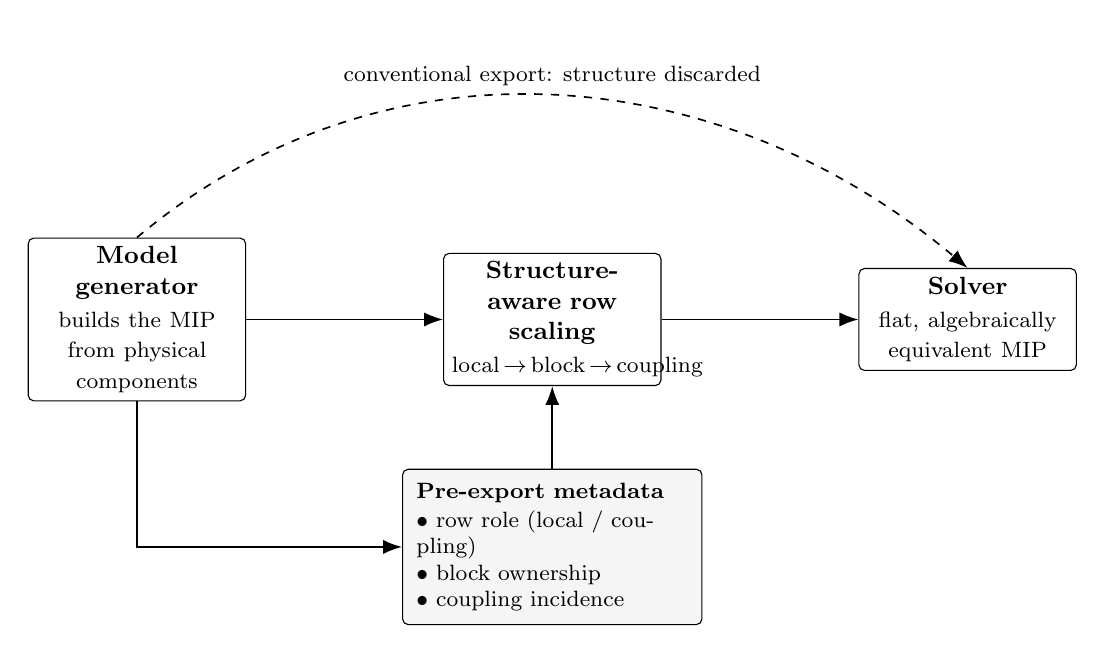
\begin{tikzpicture}[
  font=\small,
  >=Latex,
  box/.style={draw, rounded corners=2pt, align=center, minimum height=1.05cm,
              text width=2.55cm, inner sep=3pt},
  metabox/.style={draw, fill=black!4, rounded corners=2pt, align=left,
                  text width=3.45cm, inner sep=5pt, font=\footnotesize},
  arr/.style={-{Latex[length=2.4mm]}, semithick},
  darr/.style={-{Latex[length=2.4mm]}, semithick, dashed}
]
  \node[box] (gen) {\textbf{Model generator}\\[1pt]\footnotesize builds the MIP from
                    physical components};
  \node[box, right=2.5cm of gen] (scale) {\textbf{Structure-aware row scaling}\\[1pt]
                    \footnotesize local\,$\to$\,block\,$\to$\,coupling};
  \node[box, right=2.5cm of scale] (solver) {\textbf{Solver}\\[1pt]\footnotesize flat,
                    algebraically equivalent MIP};
  \node[metabox, below=1.05cm of scale] (meta) {\textbf{Pre-export metadata}\\[1pt]
                    $\bullet$ row role (local / coupling)\\
                    $\bullet$ block ownership\\
                    $\bullet$ coupling incidence};
  % main pipeline
  \draw[arr] (gen) -- (scale);
  \draw[arr] (scale) -- (solver);
  % the generator emits metadata, which keys the scaling
  \draw[arr] (gen.south) |- (meta.west);
  \draw[arr] (meta.north) -- (scale.south);
  % what a flat export throws away
  \draw[darr] (gen.north) to[out=40,in=140]
        node[above, font=\footnotesize] {conventional export: structure discarded}
        (solver.north);
\end{tikzpicture}
\caption{The proposed layer in one picture. A generator assembles the MIP from physical
components and, in doing so, knows each row's role (local or coupling), which block owns
each variable, and how coupling rows link blocks. A conventional export (dashed) hands the
solver a flat matrix in which this structure is lost. The structure-aware layer instead
reuses that pre-export metadata to choose positive row factors in a local--block--coupling
order, then exports an \emph{algebraically equivalent} MIP whose representation is better
scaled. The solver still receives a single flat matrix; only its numbers change.}
\label{fig:overview}
\end{figure}

The numerical rationale is also local--block--coupling. In an ideal block-diagonal matrix,
scalar block scaling can reduce scale separation between blocks but cannot repair a block's
intrinsic conditioning; once coupling rows are added, their relevant magnitude is their size
relative to the scaled local blocks, not their raw coefficients. Idealized conditioning
results make this precise and justify the rule's architecture, without claiming to predict
mixed-integer runtime.

We test the method on short-term hydrothermal dispatch, used not as a new formulation but as a
demanding testbed: it creates local hydro, thermal, market, shortage, and demand modules linked
by global balances, with coefficients mixing water volumes, turbine flows, power outputs, costs,
and penalties---block structure with strong scale heterogeneity. The intended generality,
however, is the generated block-structured MIP, not the hydrothermal equations. The layer
requires only metadata that many modular generators already have---which rows are local, which
block owns a variable or constraint, which global rows couple blocks---while reservoir dynamics,
turbine curves, and market costs determine the instances but never enter the scaling rule. The
hydrothermal model thus supplies a realistic stress test for a layer that targets any generated
MIP with local components and sparse global coupling.

The hydrothermal formulation used in the experiments descends from models for the
R\'io Negro hydroelectric complex and extensions to hydrothermal dispatch with Salto
Grande, developed by Risso and coauthors, together with a modular C++ implementation
used as the experimental platform
\cite{risso2025rioNegro,risso2025uruguayRiver,rodriguez2025thesis}.
We take the formulation as given and insert the proposed preprocessing layer after model
generation and before solver invocation.

The paper makes three claims of different strength: the algebraic claim is exact (positive row
scaling preserves the MIP); the numerical claim is empirical (structure-aware scaling improves
solver-facing conditioning in the tested instances); and the performance claim is conditional
(under Gurobi positive row scaling often reduces robust runtime or deterministic effort, while
under CPLEX 22.1.2.0 it does not). A controlled ablation further separates the two: the runtime
lever is a cheap per-row normalization that does not need the row-role metadata, whereas the
metadata's measured value is in the conditioning diagnostics. The method improves
representation; acceleration depends on how the solver uses it, and the rule that best
conditions the matrix is not the rule that solves fastest.

The rest of the paper follows this chain of evidence. \Cref{sec:related-work} identifies
the research niche. \Cref{sec:model} defines the generated model structure and testbed.
\Cref{sec:scaling} gives the scaling method. \Cref{sec:experimental-design} explains how
the experiments test the claims. \Cref{sec:results} reports numerical and runtime
evidence. \Cref{sec:discussion} interprets that evidence and answers likely objections.
\Cref{sec:validity} states the main limitations and reproducibility implications, and
\cref{sec:conclusion} summarizes the contribution.

\section{Related work}
\label{sec:related-work}
% -------------------------------------------------------------------------

The literature sets the stage but leaves a specific niche. Hydrothermal-dispatch models provide realistic generated block-structured MIPs with heterogeneous units and global balances; numerical-scaling work explains why coefficient magnitudes matter, but its standard tools operate on the exported matrix; and formulation-quality practice shows that algebraic representation can matter as much as the underlying set. The missing argument is narrower than ``scaling is useful'': when a generator still knows each row's role and each variable's block, that metadata can be used as numerical information before export. The resulting transformation must then be evaluated separately as an algebraic equivalence, a representation change, and a solver-dependent performance intervention.

\subsection{Hydrothermal dispatch and MIP formulations}

Hydrothermal dispatch has been studied with dynamic programming, stochastic dual
dynamic programming, nonlinear programming, and mathematical programming. Classical
references emphasize the trade-off between thermal generation costs, hydro opportunity
costs, demand satisfaction, and intertemporal reservoir management
\cite{wood2013power,conejo2010decision}. In short-term settings, MIP formulations are
attractive because they incorporate discrete decisions, piecewise-linear approximations,
local operating constraints, and system-wide balance equations in a single model
\cite{vielma2015formulation}.

This literature motivates the experimental domain but not the novelty claim. The dispatch model is used because it is a representative generated block-structured MIP: local physical modules are created separately, their variables have heterogeneous units, and a smaller set of global rows links the modules through system-wide balances. These are precisely the structural features exploited by the preprocessing layer.

\subsection{Dispatch models used in this study}

The computational experiments use a reference formulation from a research line on
MIP-based dispatch models for the Uruguayan power system. Risso et al. introduced a mixed combinatorial optimization model for the
R\'io Negro hydroelectric complex \cite{risso2025rioNegro} and extended the
modeling line to hydrothermal dispatch for the Uruguay River hydroelectric plant,
with emphasis on Salto Grande and coupled hydrothermal operation
\cite{risso2025uruguayRiver}, and an enriched formulation of the R\'io Negro model, the
closest published reference for the dispatch features used by the Full class
\cite{risso2026enriched}. The implementation used here builds on a modular
C++ version of the R\'io Negro dispatch model \cite{rodriguez2025thesis}.

This provenance fixes the scope of the experiments. The dispatch formulation, data
pipeline, and physical components are taken as given. The proposed method acts after the
model has been generated and before the solver is called. Consequently, any observed
difference between variants is attributed to an algebraically equivalent representation of
the same generated MIP, not to a modified dispatch model.

\subsection{Numerical scaling and solver-facing representation}

Scaling is a standard preprocessing operation in linear and mixed-integer optimization.
Multiplying a constraint by a positive factor preserves the feasible region but changes
the numerical magnitudes passed to the solver. These magnitudes can affect feasibility
tolerances, relaxation stability, presolve transformations, cut generation, basis quality,
and the numerical behavior of LP relaxations. Practical guidelines for difficult LP and
MIP models warn that large coefficient ranges and poor scaling can harm solver
performance even when the mathematical formulation is correct \cite{klotz2013lp,klotz2013mip}.

This paper uses that observation in a restricted way: it does not claim coefficient compression
is itself an objective, nor that a smaller coefficient range must speed up branch-and-bound. A MIP
solver is a pipeline---presolve, internal scaling, root relaxation, cuts, heuristics, incumbents,
branching, node processing, termination---whose stages can respond differently to the same
external scaling. The experiments therefore distinguish exported coefficient-range ratios from
solver-level conditioning diagnostics and from runtime, a distinction central to interpreting the
Gurobi--CPLEX contrast.

\subsection{Generic equilibration and its limitation for generated models}

Generic equilibration procedures balance rows and columns according to matrix norms.
This is a mature subfield of numerical linear algebra. Geometric-mean and
arithmetic-mean ($\ell_\infty$) scaling normalize each row or column by an average of its
coefficient magnitudes \cite{tomlin1975scaling}; Curtis--Reid scaling chooses logarithmic
diagonal factors that minimize a least-squares measure of coefficient spread
\cite{curtisreid1972}; Sinkhorn--Knopp iteration drives a nonnegative matrix toward a
doubly stochastic form by alternating row and column normalization \cite{sinkhorn1967};
and Ruiz-type scaling iteratively equilibrates row and column norms through diagonal
transformations \cite{ruiz2001scaling}. These methods are the standard tools and are
already embedded in solver presolve and internal scaling \cite{achterberg2020presolve}.
Their computational payoff, however, is known to be irregular: the largest empirical study
of LP scaling to date found that no scaling method consistently improves---and can even
degrade---simplex performance across solvers \cite{elble2012scaling}, an early warning that
coefficient compression alone is not the lever.
Such methods are useful because they are model-agnostic and can be applied after export.
That strength is also their limitation in the setting considered here. A flat-matrix method
can see coefficient magnitudes and sparsity, but it is not told whether a row is a local
turbine restriction, a thermal bound, a market-cost relation, a shortage constraint, or a
system-wide balance.

Against this background, the proposed rule is not a new equilibration kernel: its local row
factor is, in isolation, a geometric mean of the per-row coefficient extremes, as in
geometric-mean scaling. What is new is \emph{where the scales come from and in what order}---the
factors are keyed to generator metadata (row role, block ownership, coupling incidence) rather
than the flat matrix, and applied in a local--block--coupling order so coupling rows are
normalized relative to the already-scaled blocks they connect, not their raw coefficients. A flat
method (Ruiz, Curtis--Reid, geometric-mean, Sinkhorn--Knopp) cannot make this
local-versus-coupling distinction, because role information is exactly what export discards. Concretely, take two rows with
identical coefficients: a flat method cannot tell them apart and scales them identically, whereas the
structure-aware rule need not. If one is a local block row and the other a coupling row, the
local row is scaled by its own coefficients while the coupling row is scaled relative to the
\emph{already-scaled} blocks it links---so a coupling row with small raw coefficients can still
receive a large factor when it joins a poorly scaled block, and conversely. Identical numbers,
different roles, different factors: that is the lever a flat matrix cannot expose. The
model stays monolithic, as with generic scaling: an external, auditable layer that uses
generator metadata before the exported matrix loses it.

\subsection{Formulation quality, generated structure, and decomposition}

The MIP literature also stresses that formulation quality matters: two algebraically
related formulations can describe the same modeling intention but lead to different
relaxations, numerics, and search behavior \cite{vielma2015formulation}. The present
work is adjacent to that tradition but changes a different object. It does not strengthen
the formulation, add valid inequalities, alter variables, or change the feasible set. It
changes only the positive row multipliers applied to complete constraints.

The method is also adjacent to structural decomposition. Like Dantzig--Wolfe, Benders, or
Lagrangian approaches, it recognizes local blocks and global linking rows. Unlike those
methods, it does not decompose the optimization problem, introduce a master problem, or
exchange prices or cuts between subproblems. The solver still receives one monolithic MIP.
The use of block structure is numerical rather than algorithmic decomposition: block
metadata guide the representation presented to the solver.

\subsection{Remaining niche}

The resulting contribution is deliberately narrow: it tests whether local rows, block scales, and
coupling rows should be treated as different numerical objects before a generated block-structured MIP
is exported. The performance comparison rests on distributional evidence over heterogeneous
instances rather than a single runtime average, using performance profiles
\cite{dolan2002performance}, paired tests, deterministic-effort metrics, and solver-level
conditioning diagnostics.

\section{Materials and methods: generated modular formulation and testbed}
\label{sec:model}
% -------------------------------------------------------------------------

We now define the objects that the scaling rule changes and the objects it must leave
unchanged. The generator supplies the block structure; the preprocessing layer changes the
row magnitudes; the solver then receives an algebraically equivalent MIP. The dispatch
model itself is not new. What matters here is the structure that the generator exposes and
the original scale in which all feasibility and objective checks are evaluated after the
solve. We consider generated modular MIP instances formulated as
\begin{equation}
\begin{aligned}
  \min_{x} \quad & c^\top x \\
  \text{s.t.} \quad & Ax \le b, \\
  & x_j \in \Z, \qquad j \in \mathcal{I}, \\
  & x_j \in \R, \qquad j \notin \mathcal{I}.
\end{aligned}
\label{eq:generic-mip}
\end{equation}
In the general generated setting, the vector $x$ collects all variables created by the
modules, while $A$ and $b$ contain both local component constraints and global linking
constraints. In the hydrothermal testbed used here, $x$ includes generation, reservoir,
flow, spillage, shortage, and operating variables. Equalities are represented either
explicitly or by pairs of inequalities, depending on the solver interface.

The notation is intentionally application-agnostic: the layer uses the generator's structural
map---row role, block ownership, coupling incidence---not hydrological, thermal, or economic
semantics. The hydrothermal variables above explain the physical origin of the coefficients;
they are not assumptions of the scaling method.

\subsection{Hydrothermal dispatch testbed and scope}

The computational testbed uses the reference model generated by the modular dispatch
platform developed around R\'io Negro and Salto Grande hydrothermal dispatch models
\cite{risso2025rioNegro,risso2025uruguayRiver,rodriguez2025thesis}.
The application is useful because it exhibits the target structure: local modules
with heterogeneous physical units and global rows that couple those modules through
system-wide balances. The hydraulic, thermal, and market-cost constraints are those of
the reference model and its implementation.

A caveat about those heterogeneous units is in order, because it is tempting to read the
imbalance as artificial. Unit heterogeneity (reservoir volumes in $\mathrm{hm}^3$, flows in
$\mathrm{m}^3/\mathrm{s}$, power in MW) lives on the \emph{columns}, and rescaling units is,
mathematically, column scaling: an exact reformulation for continuous variables that cannot
touch integer columns at all ($x\in\mathbb{Z}$ with $x=s\,x'$ breaks integrality), so in a MIP
unit normalization is necessarily partial. Our column-normalizing baseline (\methodRuizCols{})
is in fact the weakest variant in runtime, and the base is no ill-scaled straw man: it already
runs under the solver's own internal equilibration (\cref{subsec:internal-scaling}). The lever
that moves runtime in this testbed is therefore on the rows, not the units; the row-only
scoping decision is revisited as a limitation in \cref{sec:validity}.

The method acts on the generated algebraic model, not the physical dispatch formulation: every transformation must preserve the feasible set and let objective values, constraint violations, and operational variables be read in the original scale after solution. It never uses a hydro-specific rule (reservoir priority, turbine efficiency, unit commitment) to choose factors---those details generate the rows, and only their structural role in the block-coupled MIP is used afterward.

\subsection{Block structure}

The method targets models generated by components or agents. Each component
$i\in\mathcal{B}$ creates local variables $x_i$, contributes local constraints
$A_i x_i\le b_i$, and appears in a smaller number of global constraints. Let
$\mathcal{R}_i$ denote the local row index set of component $i$. In the hydrothermal
testbed, these components include hydro, thermal, market, and demand modules. If $u_{\mathrm{loc}}$ stacks all local variables and $g$ denotes an aggregate
coupling variable, the row structure can be written schematically as
\begin{equation}
\begin{bmatrix}
D & 0 \\
0 & I_T \\
L & -I_T
\end{bmatrix}
\begin{bmatrix}
u_{\mathrm{loc}} \\
g
\end{bmatrix}
\sim
\begin{bmatrix}
b \\
d \\
0
\end{bmatrix},
\qquad
D=\diag(A_1,\ldots,A_B).
\label{eq:compact-dispatch-structure}
\end{equation}
The first block contains local component restrictions. The second block represents an
aggregate system restriction. The third block contains coupling equations that link local
component decisions with the aggregate system variable. In the dispatch application,
these rows correspond to demand and balance relationships. More generally, absorbing the
aggregate variable and its defining rows into the coupling block, the coefficient matrix
takes the block form
\begin{equation}
A =
\begin{bmatrix}
A_1 & 0   & \cdots & 0 \\
0   & A_2 & \cdots & 0 \\
\vdots & \vdots & \ddots & \vdots \\
0   & 0   & \cdots & A_B \\
L_1 & L_2 & \cdots & L_B
\end{bmatrix},
\qquad
b =
\begin{bmatrix}
b_1\\ b_2\\ \vdots\\ b_B\\ h
\end{bmatrix}.
\label{eq:block-matrix}
\end{equation}
The matrices $A_i$ encode local restrictions. The matrices $L_i$ encode each block's contribution to the global coupling rows, such as demand balance in the hydrothermal
testbed.

This structure suggests three scaling decisions: scale local rows inside each block; compute representative block scales after local row scaling; and scale global coupling rows with those block scales. The goal is to reduce harmful scale heterogeneity without erasing the modular meaning of the formulation.

\subsection{Algebraic equivalence and spectral diagnostics}
\label{subsec:equivalence-diagnostics}

We restrict the preprocessing layer to positive row scalings. This restriction makes the
transformation auditable: variables keep their original units, and the generated MIP remains
the same optimization problem. Let $D_r=\diag(d_1,\ldots,d_m)$, with $d_r>0$ for every
row. We replace $(A,b)$ by
\begin{equation}
\widetilde A = D_r A,
\qquad
\widetilde b = D_r b .
\label{eq:row-scaling}
\end{equation}
For every vector $x$,
\begin{equation}
Ax\le b
\quad\Longleftrightarrow\quad
D_rAx\le D_rb,
\label{eq:row-scaling-equivalence}
\end{equation}
because each component of the inequality is multiplied by a strictly positive scalar.
Thus positive row scaling preserves the feasible set, the integer restrictions, and the
objective function. Any difference observed after preprocessing must therefore come from
the numerical representation seen by the solver, not from a different mathematical MIP.

The theoretical arguments below use the spectral condition number as a diagnostic of linear-algebraic sensitivity. For a real matrix $M$, define
\begin{equation}
\kappa_2(M)=
\frac{\sigma_{\max}(M)}{\sigma_{\min}^{+}(M)},
\label{eq:spectral-condition}
\end{equation}
where $\sigma_{\max}(M)$ is the largest singular value and $\sigma_{\min}^{+}(M)$ is the
smallest positive singular value. For rectangular matrices, this ratio is used only as a
diagnostic over the nonzero singular spectrum; in the square benchmarks below the minimum
is taken over the full spectrum, so that singularity is reported as an infinite condition
number. This diagnostic does not characterize the full difficulty of a MIP. A MIP solver also depends on presolve, cuts, branching, primal heuristics, incumbent discovery, feasibility tolerances, and integrality. The role of $\kappa_2$ is narrower: it provides an idealized matrix argument explaining why local rows and coupling rows should not be scaled in exactly the same way.

\subsection{Ideal block scaling}
\label{subsec:ideal-block-scaling}

The block structure is not only a modeling convenience. It identifies what scalar scaling
can and cannot repair. In a purely block-diagonal matrix $D=\diag(A_1,\ldots,A_B)$, a
single scalar per block can remove differences of scale between blocks, but it cannot
improve the intrinsic conditioning of an individual block. The following benchmark makes
this statement precise in the ideal square nonsingular case.

\begin{proposition}[Ideal scalar scaling of block-diagonal matrices]
\label{prop:ideal-block-scaling}
Let $D=\diag(A_1,\ldots,A_B)$, where every $A_i$ is square and nonsingular. Let
$M_i=\sigma_{\max}(A_i)$ and $m_i=\sigma_{\min}(A_i)>0$. Then
\begin{equation}
\min_{\alpha_i>0}
\kappa_2\!\left(\diag(\alpha_1 I,\ldots,\alpha_B I)D\right)
=
\max_i \kappa_2(A_i).
\label{eq:ideal-block-minimax}
\end{equation}
One minimizer is
\begin{equation}
\alpha_i=\frac{1}{\sqrt{M_i m_i}}
=
\frac{1}{\sqrt{\sigma_{\max}(A_i)\sigma_{\min}(A_i)}} .
\label{eq:ideal-block-factor}
\end{equation}
\end{proposition}

\begin{proof}
For fixed positive scalars $\alpha_i$, the scaled matrix is block diagonal:
\begin{equation*}
\diag(\alpha_1 I,\ldots,\alpha_B I)D
=
\diag(\alpha_1 A_1,\ldots,\alpha_B A_B).
\end{equation*}
The singular values of a block-diagonal matrix are the union of the singular values of
its blocks. Therefore, for every $i$,
\begin{equation*}
\kappa_2\!\left(\diag(\alpha_1 A_1,\ldots,\alpha_B A_B)\right)
\ge
\kappa_2(\alpha_i A_i)
=
\kappa_2(A_i).
\end{equation*}
Taking the maximum over $i$ gives the lower bound
\begin{equation*}
\kappa_2\!\left(\diag(\alpha_1 A_1,\ldots,\alpha_B A_B)\right)
\ge
\max_i \kappa_2(A_i)
\end{equation*}
for every admissible block scaling.

Now choose $\alpha_i=(M_i m_i)^{-1/2}$. Then the largest and smallest singular values of
$\alpha_i A_i$ are
\begin{align*}
\sigma_{\max}(\alpha_i A_i)
&=\sqrt{\frac{M_i}{m_i}}=\sqrt{\kappa_2(A_i)},\\
\sigma_{\min}(\alpha_i A_i)
&=\sqrt{\frac{m_i}{M_i}}=\frac{1}{\sqrt{\kappa_2(A_i)}}.
\end{align*}
Because the singular values of the complete block-diagonal matrix are obtained by
pooling the singular values of its blocks,
\begin{equation*}
\sigma_{\max}\!\left(\diag(\alpha_1 A_1,\ldots,\alpha_B A_B)\right)
=
\sqrt{\max_i \kappa_2(A_i)},
\end{equation*}
and
\begin{equation*}
\sigma_{\min}\!\left(\diag(\alpha_1 A_1,\ldots,\alpha_B A_B)\right)
=
\frac{1}{\sqrt{\max_i \kappa_2(A_i)}}.
\end{equation*}
The resulting condition number is $\max_i\kappa_2(A_i)$, matching the lower bound.
\end{proof}

This proposition is not used as an algorithmic recipe. The generated MIPs considered in
this paper contain rectangular local matrices, inequalities, bounds, redundant rows, and
integer variables; computing singular-value-based block scalings would not be a practical
external preprocessing rule for the exported MIP. The proposition instead justifies the
architecture of the method. First, poor scale separation between blocks should be treated
differently from poor conditioning inside a block. Second, after local row scaling, each
block should contribute a representative scale before global coupling rows are processed.
The implemented rules therefore replace the ideal singular-value quantities
$(M_i,m_i)$ with coefficient-based proxies that are cheap to compute from the generated
model. These propositions are design principles, not performance theorems. They should not be read as predictive guarantees for the implemented
MIP preprocessing rule; they motivate the distinction between local rows, block scales,
and coupling rows.

\subsection{Effect of global coupling rows}
\label{subsec:global-coupling-theory}

Local block scaling does not exhaust the numerical issue because the generated model is
not purely block diagonal. In the hydrothermal dispatch testbed, global rows couple local
agent decisions through demand and balance equations. The relevant schematic block is
\begin{equation}
A_{\mathrm{bal}}=
\begin{bmatrix}
D & 0\\
L & -I_T
\end{bmatrix},
\label{eq:balance-block-matrix}
\end{equation}
where $D=\diag(A_1,\ldots,A_B)$ represents the local blocks and $L$ collects the
coefficients by which local decisions enter the global balance. If $D$ is nonsingular, then
\begin{equation}
A_{\mathrm{bal}}=
\begin{bmatrix}
I & 0\\
LD^{-1} & -I_T
\end{bmatrix}
\begin{bmatrix}
D & 0\\
0 & I_T
\end{bmatrix}.
\label{eq:balance-factorization}
\end{equation}
This factorization separates local scale from coupling scale. The matrix $L$ by itself is
not the relevant object: the coupling felt by the balance row after the local block scales
are taken into account is $LD^{-1}$. Thus a row with moderate entries in $L$ can still be
numerically influential if some local block contains weak directions.

The next result makes the dependence on the effective coupling norm explicit.

\begin{proposition}[Conditioning of a triangular coupling factor]
\label{prop:triangular-coupling}
Let $R\in\R^{m\times n}$ and define
\begin{equation}
T_R=
\begin{bmatrix}
I_n & 0\\
R & I_m
\end{bmatrix}.
\end{equation}
If $\rho=\norm{R}_2$, then
\begin{equation}
\kappa_2(T_R)=
\left(\frac{\sqrt{\rho^2+4}+\rho}{2}\right)^2 .
\label{eq:link-condition}
\end{equation}
The sign of the identity block is immaterial: since
$\bigl[\begin{smallmatrix}I&0\\R&-I\end{smallmatrix}\bigr]
=\diag(I,-I)\bigl[\begin{smallmatrix}I&0\\-R&I\end{smallmatrix}\bigr]$ and orthogonal
factors preserve singular values, the same formula applies to the factor with $-I_T$ in
\cref{eq:balance-factorization}.
\end{proposition}

\begin{proof}
Let $R=U\Sigma V^\top$ be a singular value decomposition (SVD) of $R$, with $U$ and $V$
orthogonal. Orthogonal multiplication does not change singular values, and hence
$T_R$ has the same singular values as
\begin{equation*}
\begin{bmatrix}
V^\top & 0\\
0 & U^\top
\end{bmatrix}
\begin{bmatrix}
I_n & 0\\
R & I_m
\end{bmatrix}
\begin{bmatrix}
V & 0\\
0 & U
\end{bmatrix}
=
\begin{bmatrix}
I_n & 0\\
\Sigma & I_m
\end{bmatrix}.
\end{equation*}
For each singular value $\sigma$ of $R$, the nontrivial part reduces to the two-dimensional
block
\begin{equation*}
B_\sigma=
\begin{bmatrix}
1 & 0\\
\sigma & 1
\end{bmatrix}.
\end{equation*}
The squared singular values of $B_\sigma$ are the eigenvalues of
\begin{equation*}
B_\sigma^\top B_\sigma=
\begin{bmatrix}
1+\sigma^2 & \sigma\\
\sigma & 1
\end{bmatrix},
\end{equation*}
namely
\begin{equation*}
\lambda_{\pm}(\sigma)=
\frac{\sigma^2+2\pm \sigma\sqrt{\sigma^2+4}}{2}.
\end{equation*}
Their product is one, and $\lambda_+(\sigma)$ is increasing for $\sigma\ge0$. Additional
directions associated with zero singular values of $R$ contribute singular values equal to
one. Therefore the largest squared singular value of $T_R$ is $\lambda_+(\rho)$ and the
smallest squared singular value is $1/\lambda_+(\rho)$. Consequently,
\begin{align*}
\kappa_2(T_R)
&=\lambda_+(\rho)\\
&=\frac{\rho^2+2+\rho\sqrt{\rho^2+4}}{2}\\
&=\left(\frac{\sqrt{\rho^2+4}+\rho}{2}\right)^2 .
\end{align*}
\end{proof}

Applied to \eqref{eq:balance-factorization}, the proposition shows that the balance row
should not be treated as an ordinary local row. Its numerical effect depends on the
effective coupling proxy $\norm{LD^{-1}}_2$, not only on the raw magnitude of the
entries in $L$. Moreover, if a common positive factor $\gamma$ is applied to the coupling
row, the scaled block satisfies
\begin{equation}
\begin{bmatrix}
D & 0\\
\gamma L & -\gamma I_T
\end{bmatrix}
=
\begin{bmatrix}
I & 0\\
\gamma LD^{-1} & -I_T
\end{bmatrix}
\begin{bmatrix}
D & 0\\
0 & \gamma I_T
\end{bmatrix}.
\label{eq:scaled-balance-factorization}
\end{equation}
Thus $\gamma$ changes both the effective coupling term and the relative scale of the
aggregate variable in the balance equation: pushing $\gamma$ down improves the triangular
factor of \cref{eq:scaled-balance-factorization} but degrades its diagonal factor, and
vice versa. This is the trade-off behind the proposed coupling treatment---global rows
are scaled after local rows, using block-level representative scales, rather than by an
isolated row norm---and the augmented rule resolves it explicitly by minimizing the
product of the two factors (\cref{eq:augmented-coupling-factor} in
\cref{subsec:strategy-1}). In the implemented variants, $D^{-1}$ and singular values are
replaced by coefficient-based block proxies, yielding a cheap operational approximation
to the ideal coupling measure.


\subsection{From ideal diagnostics to implementable proxies}
\label{subsec:ideal-to-proxies}

The two propositions establish \emph{which} numerical distinctions a structure-aware
rule must preserve, and thereby justify the architecture. They imply three design
requirements: local scale imbalance should be reduced before global coupling rows are
diagnosed; blocks should be summarized only after their local rows are on a comparable
scale; and a coupling row should be scaled relative to the blocks it connects, not only
relative to its own raw coefficient norm. The implemented method realizes exactly these
distinctions through coefficient-based proxies: they are cheap to compute from the
generated model before export, auditable because they depend only on visible row and
block metadata, and they avoid expensive or unstable singular-value information from the
rectangular, redundant, inequality-based matrices that arise in generated MIPs. The row
factor based on the geometric mean of the smallest and largest nonzero magnitudes is a
robust coefficient-scale proxy that centers each eligible row without changing variables,
bounds, integrality, or the objective.

The coupling rule implements the same logic. In \cref{prop:triangular-coupling}, the
relevant ideal object is the effective coupling magnitude after local scaling, a term of
the form $LD^{-1}$; since generated blocks are rectangular, possibly redundant, and not
inverted by the preprocessing layer, the block scale $s_i$ used below is a representative
coefficient scale for block $i$ computed after local row scaling, and the coupling proxy
divides each coupling coefficient by the representative scale of the block owning its
column. This is a cheap, auditable surrogate for asking whether the coupling row is large
relative to the local numerical scale of the blocks it links.

We state the scope of this argument once and plainly: the propositions describe square,
nonsingular blocks under exact SVD scaling, the proxies act on rectangular,
inequality-based matrices, and we establish no bound relating the proxy scale to the
ideal spectral factor in \cref{prop:ideal-block-scaling}. The propositions therefore
motivate the design, and its empirical validity is verified directly in the controlled
synthetic suite of \cref{subsec:synthetic-benchmark}, where blocks are small, singular
values are cheap to compute, and conditioning is measurable by construction.

This bridge also explains why the proposed method is row-based. Positive row scaling
preserves the original units and domains of all variables; integer and binary variables do
not require reinterpretation, and objective coefficients are left in their original
economic units. Column scaling can be useful as a generic numerical device, so a
Ruiz-plus-column baseline is included in the experiments. It is not part of the proposed
structure-aware layer because the central claim is that row-role and coupling metadata
alone already provide useful pre-export numerical information while keeping the
transformation algebraically transparent.


% -------------------------------------------------------------------------
\section{Numerical scaling method}
\label{sec:scaling}
% -------------------------------------------------------------------------

The scaling method keeps the same structural roles visible throughout: local rows, blocks, and coupling rows. Local rows receive row factors first. Blocks then inherit representative scales from their scaled local rows. Coupling rows receive their factors last, using the blocks they connect. This order is the algorithmic expression of the numerical argument in \cref{subsec:ideal-block-scaling,subsec:global-coupling-theory} and of the proxy interpretation in \cref{subsec:ideal-to-proxies}.

This section defines the numerical transformations tested in the results. The base variant is the unscaled model generated by the platform. The two proposed variants use the same local--block--coupling architecture but differ in whether the right-hand side participates in the scale diagnosis. Ruiz-type variants provide generic flat-matrix baselines. This organization makes two contrasts explicit. The comparison between \methodAug{} and \methodMat{} isolates the role of right-hand-side information within the same architecture; the comparison with Ruiz-type baselines tests whether generator-level row roles add information beyond generic flat-matrix equilibration.

\subsection{Base formulation}

The \methodBase{} variant is passed to the solver without external scaling. Internal
solver presolve and internal scaling remain enabled unless stated otherwise. All
speedups, objective deviations, and equivalence checks are computed relative to this
variant on the same instance, solver, and gap setting.

\subsection{Augmented structure-aware scaling}
\label{subsec:strategy-1}

The first proposed variant, denoted \methodAug{}, computes row factors from both
coefficient magnitudes and right-hand sides. The motivation is that a generated row may
have moderate coefficients but a right-hand side in a very different physical or economic
scale. Such a row can still lead to a poorly balanced numerical representation.

For each local row $r$, define
\begin{equation}
\mathcal{S}_r^{A,b}
=
\left\{
\abs{a_{rj}}: a_{rj}\neq 0
\right\}
\cup
\left\{
\abs{b_r}: b_r\neq 0
\right\}.
\label{eq:augmented-set}
\end{equation}
If $\mathcal{S}_r^{A,b}\neq\emptyset$, let
\begin{equation}
M_r^{A,b}=\max \mathcal{S}_r^{A,b},
\qquad
m_r^{A,b}=\min \mathcal{S}_r^{A,b}.
\label{eq:augmented-extremes}
\end{equation}
The local row factor is
\begin{equation}
\alpha_r^{A,b}=\frac{1}{\sqrt{M_r^{A,b}m_r^{A,b}}}.
\label{eq:alpha-augmented}
\end{equation}
The scaled row is
\begin{equation}
\alpha_r^{A,b}a_r^\top x\le \alpha_r^{A,b}b_r.
\end{equation}

The augmented rule is not only a row-by-row normalization. It is a three-stage
structure-aware procedure that first rescales local rows, then summarizes the resulting
local block scales, and finally uses those block scales to treat coupling rows separately.
After local scaling, let $\widetilde a_{rj}=\alpha_r^{A,b}a_{rj}$ for local rows. For each
local block $i$, define
\begin{equation}
M_i^{A,b}
=
\max_{r\in\mathcal{R}_i,\,j:\,\widetilde a_{rj}\neq 0}
\abs{\widetilde a_{rj}},
\qquad
m_i^{A,b}
=
\min_{r\in\mathcal{R}_i,\,j:\,\widetilde a_{rj}\neq 0}
\abs{\widetilde a_{rj}}.
\label{eq:augmented-block-extremes}
\end{equation}
The representative scale of block $i$ is
\begin{equation}
s_i^{A,b}=\sqrt{M_i^{A,b}m_i^{A,b}}.
\label{eq:augmented-block-scale}
\end{equation}
For a coupling row $r$, let $\beta(j)$ denote the local block that owns column $j$;
columns owned by no block enter at the mean block scale, and components that contribute
no local rows enter at unit scale. The effective coupling proxy of row $r$ is
\begin{equation}
\widehat\rho_r^{A,b}
=
\sqrt{
\sum_j
\left(
\frac{\abs{a_{rj}}}{s_{\beta(j)}^{A,b}}
\right)^2
},
\label{eq:augmented-coupling-rho}
\end{equation}
the magnitude of the row relative to the representative scales of the blocks it connects,
and $\rho=\max_r \widehat\rho_r^{A,b}$ is the worst such magnitude over the coupling
rows. \methodAug{} then scales the coupling block by a \emph{single} factor
$\gamma^{A,b}$, applied to every coupling row and chosen to minimize the conditioning
surrogate that the idealized analysis suggests:
\begin{equation}
\gamma^{A,b}=\argmin_{\gamma}\,\Phi(\gamma),
\qquad
\Phi(\gamma)=\kappa_T(\gamma\rho)\,\kappa_B(\gamma),
\qquad
\kappa_B(\gamma)=\frac{\max(\bar M,\gamma)}{\min(\bar m,\gamma)},
\label{eq:augmented-coupling-factor}
\end{equation}
where $\kappa_T(\cdot)$ is exactly $\kappa_2$ of the triangular coupling factor
(\cref{eq:link-condition}), $\kappa_B$ is the diagonal spread once the aggregate variable
enters at scale $\gamma$, and, writing $\kappa_i=M_i^{A,b}/m_i^{A,b}$ for the
post-local-normalization coefficient spread of block $i$,
\begin{equation}
\bar M=\max_i\sqrt{\kappa_i},\qquad \bar m=\min_i\tfrac{1}{\sqrt{\kappa_i}},
\label{eq:augmented-diagonal-spread}
\end{equation}
the extremal coefficient magnitudes across blocks after local scaling---the conditioning
proxy of the diagonal factor $\widetilde D$, not the block scale $s_i^{A,b}$ of
\cref{eq:augmented-block-scale}, which enters only the coupling proxy $\widehat\rho_r$.
The minimizer is found on a logarithmic grid
$\gamma\in[10^{-6},10^{6}]$, and the stage is skipped when the effective coupling is
already moderate ($\rho$ below a fixed threshold) or when the minimizer falls inside the
near-identity band of the safeguards. The grid search resolves explicitly the trade-off
exposed by \cref{eq:scaled-balance-factorization}: decreasing $\gamma$ improves the
triangular factor but degrades the diagonal one, and, by submultiplicativity of $\kappa_2$
over that factorization, $\kappa_2$ of the scaled balance block is at most
$\kappa_T(\gamma\rho)\,\kappa_B(\gamma)=\Phi(\gamma)$, so minimizing $\Phi$ minimizes this
upper bound. The released implementation evaluates these proxies from
coefficient summaries of the generated model; the exact evaluation order is documented in
the reproducibility repository.
This sequence is the
main structural feature of the proposed method: local physical scales are used first,
block scales are estimated after local normalization, and global coupling rows are scaled
only after the blocks they connect have been put on comparable numerical footing.

\subsection{Matrix-only structure-aware scaling}
\label{subsec:strategy-2}

The second proposed variant, denoted \methodMat{}, uses the same row--block--coupling
architecture but excludes $b$ from the diagnosis. The right-hand side is still multiplied
by the selected row factor to preserve equivalence, but it does not influence factor
selection.

For each local row $r$, define the nonzero coefficient extremes
\begin{equation}
M_r^{A}=\max_{j:\,a_{rj}\neq 0}\abs{a_{rj}},
\qquad
m_r^{A}=\min_{j:\,a_{rj}\neq 0}\abs{a_{rj}}.
\label{eq:matrix-row-extremes}
\end{equation}
If the row has at least one nonzero coefficient, the row factor is
\begin{equation}
\alpha_r^{A}=\frac{1}{\sqrt{M_r^{A}m_r^{A}}}.
\label{eq:matrix-row-factor}
\end{equation}
The scaled row is
\begin{equation}
\alpha_r^{A}a_r^\top x\le \alpha_r^{A}b_r.
\end{equation}
This factor centers the smallest and largest nonzero coefficient magnitudes of the row
around a common scale. Unlike Euclidean-norm scaling, it does not directly depend on
the number of nonzeros in the row.

Let $\widetilde a_{rj}=\alpha_r^A a_{rj}$ after local row scaling. For each local block
$i$, define
\begin{equation}
M_i^{A}
=
\max_{r\in\mathcal{R}_i,\,j:\,\widetilde a_{rj}\neq 0}
\abs{\widetilde a_{rj}},
\qquad
m_i^{A}
=
\min_{r\in\mathcal{R}_i,\,j:\,\widetilde a_{rj}\neq 0}
\abs{\widetilde a_{rj}}.
\label{eq:matrix-block-extremes}
\end{equation}
The representative block scale is
\begin{equation}
s_i^A=\sqrt{M_i^A m_i^A}.
\label{eq:matrix-block-scale}
\end{equation}
No additional multiplier is applied to all rows or columns of block $i$ at this stage.
The quantity $s_i^A$ is an auxiliary representative scale: it is used only to
normalize the contribution of block $i$ when the coupling-row proxy is computed.

For a coupling row $r$, with the same ownership map $\beta(\cdot)$ and the same
convention for blockless columns as in \cref{subsec:strategy-1}, define
\begin{equation}
\widehat{\rho}_r^{A}
=
\sqrt{
\sum_j
\left(
\frac{\abs{a_{rj}}}{s_{\beta(j)}^{A}}
\right)^2
}.
\label{eq:matrix-coupling-rho}
\end{equation}
If $\widehat{\rho}_r^{A}>0$, the coupling-row factor is per row,
\begin{equation}
\gamma_r^{A}=\frac{1}{\widehat{\rho}_r^{A}},
\label{eq:matrix-coupling-factor}
\end{equation}
clipped to $[10^{-8},10^{8}]$ and subject to the safeguards below. When the block
extremes of \cref{eq:matrix-block-extremes} are computed, the implementation restricts
them to coefficients inside a fixed moderation window $(10^{-6},10^{6})$, so a single
extreme coefficient cannot distort $s_i^A$.

The comparison between \methodAug{} and \methodMat{} isolates the empirical value of
including the right-hand side in the scaling diagnosis. Both variants preserve the same
structural architecture; they differ only in whether $b$ participates in factor selection.

\subsection{Safeguards}

All applied scaling factors---the local row factors and the coupling-row factors in the
augmented or matrix-only variants---are subject to two per-factor safeguards, applied
independently to each factor. The representative block scales $s_i$ are auxiliary
quantities used to compute coupling-row proxies; they are not applied as independent
row or column scalings.

\paragraph{Near-identity threshold}
A factor is applied only if it departs from one by at least a factor of $u=2$; factors
falling in the open band $(1/u,\,u)=(0.5,\,2)$ are treated as negligible and skipped:
\begin{equation}
\theta \text{ is applied}
\iff
\left(\theta \le \frac{1}{u}\right)\ \text{or}\ \left(\theta \ge u\right),
\qquad u=2 .
\label{eq:near-identity}
\end{equation}
This prevents re-scaling rows or coupling rows that are already at a reasonable scale.

\paragraph{Admissible coefficient range}
A factor is applied only if it keeps every affected coefficient within the window
$[\varepsilon_{\min},\varepsilon_{\max}] = [10^{-9},\,10^{9}]$. Writing
$c_{\min}$ and $c_{\max}$ for the smallest and largest magnitudes of the affected
coefficients, the factor $\theta$ is admitted only if
\begin{equation}
\begin{aligned}
\varepsilon_{\min} &\le c_{\min}\,\theta,
& c_{\max}\,\theta &\le \varepsilon_{\max},\\
[\varepsilon_{\min},\varepsilon_{\max}]&=[10^{-9},\,10^{9}].
\end{aligned}
\label{eq:coef-window}
\end{equation}
Otherwise, the factor is not applied and the corresponding row or coupling row is left at its base scale. The coupling factor is additionally hard-clipped to
$\gamma \in [10^{-8},\,10^{8}]$ prior to this check.

Because each admitted factor is a strictly positive multiplier applied to a complete
constraint---both its coefficients and its right-hand side---the feasible set and the
objective value are preserved exactly. The safeguards therefore restrict only the
numerical aggressiveness of the transformation, never its equivalence to the base model.


\subsection{Ruiz-type baselines}

We compare the proposed variants with two generic baselines. The first,
\methodRuiz{}, applies iterative row equilibration based on the maximum norm. The
second, \methodRuizCols{}, combines Ruiz-type row equilibration with continuous-column
scaling and physical normalization. These baselines separate the effect of generic
coefficient compression from the effect of exploiting model structure.

\methodRuiz{} is deliberately not a weak foil: max-norm equilibration is a standard, strong
flat-matrix scheme, and \methodRuizCols{} additionally grants it the column-scaling lever the
structure-aware rule forgoes. The baselines isolate a narrow question---whether row roles and
coupling incidence carry numerical information that a flat-matrix equilibrator, however well
tuned, cannot recover once export has discarded them; the separate ``could the solver have done
this itself'' control is the internal-scaling baseline of \cref{subsec:internal-scaling}. Every
variant hands the solver the same monolithic MIP; only the pre-export row factors differ.

The final implementation uses
\begin{equation}
K=4
\end{equation}
Ruiz iterations. Binary and integer variables are not rescaled unless explicitly stated,
so that bounds, objective interpretation, and integrality remain unchanged.

\subsection{Algorithmic summary}

\Cref{alg:augmented-scaling} collects the augmented rule end to end.

\begin{algorithm}[t]
\caption{Augmented structure-aware row scaling}
\label{alg:augmented-scaling}
\begin{algorithmic}[1]
\Require Matrix $A$, right-hand side $b$, row roles (local/coupling), block ownership $\beta(\cdot)$, coupling incidence
\Ensure Scaled matrix $\widetilde A$, scaled right-hand side $\widetilde b$
\State Initialize row factors $d_r\gets 1$
\For{each local block $i\in\mathcal{B}$}
  \For{each local row $r\in\mathcal{R}_i$}
    \State Build $\mathcal{S}_r^{A,b}$ from nonzero coefficients and nonzero right-hand side
    \If{$\mathcal{S}_r^{A,b}\neq\emptyset$}
      \State Compute $M_r^{A,b}$ and $m_r^{A,b}$ using \cref{eq:augmented-extremes}
      \State Set $\alpha_r^{A,b}\gets 1/\sqrt{M_r^{A,b}m_r^{A,b}}$
      \If{the safeguards admit $\alpha_r^{A,b}$} \State Update $d_r\gets d_r\alpha_r^{A,b}$ \EndIf
    \EndIf
  \EndFor
\EndFor
\State Compute the locally scaled coefficients $\widetilde a_{rj}=d_r a_{rj}$
\State Compute block scales $s_i^{A,b}=\sqrt{M_i^{A,b}m_i^{A,b}}$ using \cref{eq:augmented-block-scale}
\State Compute $\widehat\rho_r^{A,b}$ for every coupling row using \cref{eq:augmented-coupling-rho}; set $\rho\gets\max_r\widehat\rho_r^{A,b}$
\If{$\rho$ exceeds the coupling threshold}
  \State Set $\gamma^{A,b}\gets\argmin_{\gamma}\Phi(\gamma)$ over the logarithmic grid $\gamma\in[10^{-6},10^{6}]$ (\cref{eq:augmented-coupling-factor})
  \If{$\gamma^{A,b}$ lies outside the near-identity band}
    \State Update $d_r\gets d_r\gamma^{A,b}$ for every coupling row $r$
  \EndIf
\EndIf
\State Return $\widetilde A=\diag(d)A$ and $\widetilde b=\diag(d)b$
\end{algorithmic}
\end{algorithm}

The matrix-only algorithm follows the same local and block stages with the
coefficient-only set $\{\abs{a_{rj}}:a_{rj}\neq 0\}$ and the representative block scales
and coupling proxies of \cref{eq:matrix-block-scale,eq:matrix-coupling-rho}; its coupling
stage differs in granularity, assigning each coupling row its own factor
$\gamma_r^{A}=1/\widehat\rho_r^{A}$ (\cref{eq:matrix-coupling-factor}) instead of the
single grid-selected $\gamma^{A,b}$. In the present
manuscript, \methodMat{} is interpreted as an ablation of the right-hand-side
information: it preserves the same local-row and coupling-row architecture, but the
right-hand side does not enter the factor-selection rule.

% -------------------------------------------------------------------------
\section{Experimental design}
\label{sec:experimental-design}
% -------------------------------------------------------------------------

\subsection{Instance classes and scenarios}

The experiments are organized around four reader questions: does scaling preserve the original
optimization problem, does it improve the numerical representation, does that change solver
behavior, and does the effect survive changes in class, solver, and tolerance? The study uses
three instance classes generated by the same modular hydrothermal platform, built from
operational instances with available real input data. The pools are balanced by construction:
every variant is attempted on every instance of a class (204 Simple, 68 SG-Ter-Mer, 34 Full), so
no instance is dropped for one variant and kept for another. Valid-run counts still differ
slightly across class--scenario--variant cells because individual runs can fail with an error
status (an aborted solve, a missing log, an unavailable conditioning read)---a small fraction,
about $1$--$3\%$ per class in the Gurobi scenarios, recorded per run in the artifacts. Descriptive
metrics use all valid runs for a row (so a cell may report, say, $195$--$199$ of $204$ Simple
instances), whereas speedups, tests, and all base comparisons use matched base--variant pairs in
which both runs succeeded, and are therefore unaffected by the unbalanced descriptive counts.

Each measurement is tied to the part of the argument it can support: algebraic equivalence
is checked by descaling and original-scale feasibility and integrality tests; the numerical
claim by exported coefficient-range summaries and solver-level conditioning diagnostics; the
performance claim by matched base--variant speedups, deterministic effort, performance
profiles, and primal--dual progress; and solver dependence by separate Gurobi and CPLEX
scenarios at two tolerances (the same distinctions return as claim--evidence--limitation in
\cref{tab:claim-summary}).

\begin{table*}[t]
\centering
\caption{Three instance classes test the method on progressively different generated hydrothermal models.}
\label{tab:instance-stats}
\begin{threeparttable}
\small
\begin{tabular}{@{}p{0.16\textwidth}p{0.42\textwidth}p{0.28\textwidth}r@{}}
\toprule
Class & Configuration & Main role & Instances \\
\midrule
Simple & R\'io Negro + fixed demand + fixed dispatch & Basic numerical behavior & 204 \\
Full & R\'io Negro nonlinear + Salto Grande + thermal units + market & Largest integrated model & 34 \\
SG-Ter-Mer & Salto Grande + thermal units + market & Coupled hydrothermal subset & 68 \\
\bottomrule
\end{tabular}
\begin{tablenotes}[flushleft]\footnotesize
\item The counts report the maximum operational instance pools with available real input
      data. Scenario tables may show different $n$ values because each aggregate row uses
      the valid runs available for that solver--gap--variant combination. Pairwise
      speedups and tests use matched base--variant pairs only.
\end{tablenotes}
\end{threeparttable}
\end{table*}

\noindent \Cref{tab:instance-stats} separates the three pools: Simple gives the largest
sample for distributional evidence, Full is the smallest and most integrated model, and
SG-Ter-Mer isolates a coupled hydrothermal subset---so the averages and paired tests do not come
from a single homogeneous population.

The class names are application-specific, but the contrast is structural: whether the rule behaves
consistently as the generated MIP moves from a simpler modular model to larger or more strongly
coupled ones. The conclusions are thus stated at two levels---empirical evidence from hydrothermal
dispatch, methodological object the use of generator metadata in block-structured engineering
MIPs.


We evaluate four solver--gap scenarios. The time limit is one hour per solve in every
case. Internal solver presolve and internal scaling are left enabled, because the goal is
to test whether external preprocessing helps in a realistic solver pipeline. All main
experiments were run on ClusterUY, a collaborative high-performance computing
platform for scientific computing in Uruguay \cite{nesmachnow2019clusteruy}.

\begin{table*}[t]
\centering
\caption{Four solver--tolerance scenarios separate solver dependence from gap-tolerance effects.}
\label{tab:solver-scenarios}
\begin{threeparttable}
\small
\begin{tabular}{@{}clc@{}}
\toprule
Scenario & Solver & Relative MIPGap \\
\midrule
1 & Gurobi & $10^{-2}$ \\
2 & Gurobi & $10^{-3}$ \\
3 & CPLEX  & $10^{-2}$ \\
4 & CPLEX  & $10^{-3}$ \\
\bottomrule
\end{tabular}
\begin{tablenotes}[flushleft]\footnotesize
\item Deterministic time is reported when available: \Work{} units for Gurobi and ticks
for CPLEX.
\end{tablenotes}
\end{threeparttable}
\end{table*}

\noindent The four scenarios in \cref{tab:solver-scenarios} vary two dimensions separately: the stopping tolerance and the solver pipeline. Scenarios 1--2 test Gurobi at two MIPGap values; scenarios 3--4 repeat the comparison under CPLEX and serve as a solver contrast.


\begin{table*}[t]
\centering
\caption{The computational environment fixes solver versions, time limits, and default presolve settings for all comparisons.}
\label{tab:computational-environment}
\begin{threeparttable}
\small
\begin{tabular}{@{}ll@{}}
\toprule
Item & Configuration \\
\midrule
Cluster & ClusterUY, partition \texttt{ute} \\
Processor & Intel Xeon Gold 6138 \\
Threads & 16 \\
Memory limit & 12 GB \\
Time limit & 1 hour per solve \\
Gurobi version & 13.0.1~\cite{gurobi_manual} \\
CPLEX version & 22.1.2.0~\cite{cplex_manual} \\
Presolve & solver default, enabled \\
\bottomrule
\end{tabular}
\begin{tablenotes}[flushleft]\footnotesize
\item Solver-internal scaling and presolve were left at their default enabled settings
unless otherwise stated. CPLEX 22.1.2.0 is the version available in the ClusterUY
environment used for the long runs; conclusions involving CPLEX should therefore be
interpreted as solver-version and environment specific.
\end{tablenotes}
\end{threeparttable}
\end{table*}

\noindent The configuration in \cref{tab:computational-environment} matters because the proposed preprocessing is tested on top of each solver's default numerical pipeline. The CPLEX conclusions below are therefore statements about this version and ClusterUY environment, not claims about all CPLEX releases or parameter choices.



\FloatBarrier
\subsection{Controlled synthetic block-structured benchmark}
\label{subsec:synthetic-benchmark}

The hydrothermal testbed evaluates the proposed preprocessing rule on realistic
operational generated MIPs. To complement this real-data setting, we define a controlled
synthetic benchmark whose purpose is diagnostic rather than physical. The synthetic
instances are not intended to model a power system. They isolate the numerical mechanism
targeted by the method by allowing local-row scale imbalance and coupling-row scale
imbalance to be varied independently.

Each synthetic instance consists of $B$ local blocks. Block $i$ contains continuous
activity variables $y_i\in\R^{n_y}_+$ and binary activation variables
$z_i\in\{0,1\}^{n_z}$. A nonnegative slack vector $s$ is added to the global coupling
constraints to guarantee feasibility. The generic synthetic MIP is
\begin{equation}
\begin{aligned}
\min_{y,z,s}\quad
& \sum_{i=1}^{B} c_i^\top y_i
  + \sum_{i=1}^{B} q_i^\top z_i
  + P\mathbf{1}^\top s \\
\text{s.t.}\quad
& R_i y_i + G_i z_i \le r_i,
  \qquad i=1,\ldots,B,\\
& 0 \le y_{ik} \le U_{ik}z_{ik},
  \qquad i=1,\ldots,B,\quad k=1,\ldots,n_y,\\
& \sum_{i=1}^{B} L_i y_i
  + \sum_{i=1}^{B} H_i z_i
  + s \ge d,\\
& s\ge 0,\qquad z_i\in\{0,1\}^{n_z}.
\end{aligned}
\label{eq:synthetic-mip}
\end{equation}
The first group of constraints defines local block restrictions, the second group links
continuous activity variables to binary activation variables, and the third group creates
global coupling rows. The penalty $P$ is chosen large enough that the slack variable is
used only when the activated block capacity cannot satisfy the synthetic demand.

The unscaled coefficients are generated from bounded random distributions with controlled
sparsity. Local matrices $R_i$ and $G_i$ define block-internal resource constraints.
Coupling matrices $L_i$ and $H_i$ define the contribution of each block to the global rows.
The generator records row metadata
\begin{equation}
\texttt{row\_type}\in\{\texttt{local},\texttt{coupling}\},
\qquad
\texttt{block\_id}\in\{1,\ldots,B\},
\label{eq:synthetic-row-metadata}
\end{equation}
and column metadata identifying the block associated with each variable. This metadata is
the same information required by the structure-aware scaling rules.

Scale imbalance is introduced after the clean synthetic MIP has been generated. For each
eligible row $r$, a positive row multiplier
\begin{equation}
\theta_r = 10^{\xi_r},
\qquad
\xi_r\sim\mathcal{U}[-S,S],
\label{eq:synthetic-row-factor}
\end{equation}
is drawn and applied to the entire row, including its right-hand side. Therefore, the
scaled representation is algebraically equivalent to the clean synthetic MIP. The severity
parameter $S$ controls the possible scale range. We use
\begin{equation}
S\in\{0,3,6\},
\label{eq:synthetic-severity}
\end{equation}
corresponding to no artificial imbalance, moderate imbalance, and strong imbalance.

Four scale patterns are considered:
\begin{enumerate}
  \item \textbf{None:} no artificial row scaling is applied.
  \item \textbf{Local:} only local block rows are multiplied by factors
  \eqref{eq:synthetic-row-factor}.
  \item \textbf{Coupling:} only global coupling rows are multiplied by factors
  \eqref{eq:synthetic-row-factor}.
  \item \textbf{Mixed:} both local block rows and global coupling rows are multiplied.
\end{enumerate}
The ``none'' pattern is a negative control: a useful preprocessing rule should not create
large artificial changes when the representation is already reasonably scaled. The
``local'' and ``coupling'' patterns isolate the two numerical objects distinguished by the
proposed method. The ``mixed'' pattern approximates the combined heterogeneity observed in
generated models. These controlled patterns are mechanism checks. They verify that the implementation reacts correctly when the source of imbalance is known by construction, but they are not an operational local-only versus coupling-only ablation on the real hydrothermal instances.


\begin{table*}[t]
\centering
\caption{Controlled synthetic benchmark factors isolate the numerical mechanisms targeted by the scaling rule.}
\label{tab:synthetic-design}
\begin{threeparttable}
\small
\begin{tabular}{@{}p{0.18\textwidth}p{0.20\textwidth}p{0.26\textwidth}p{0.27\textwidth}@{}}
\toprule
Factor & Levels used & Controlled object & Purpose \\
\midrule
Scale pattern & none, local, coupling, mixed
& Row class affected by artificial scaling
& Separate local imbalance from coupling imbalance \\
Severity $S$ & $0,3,6$
& Range of row multipliers $10^{-S}$--$10^S$
& Test mild and severe numerical heterogeneity \\
Blocks and size & $B=10$, $n_y=n_z=8$
& Number and size of generated local components
& Keep a fixed block structure while varying row-scale imbalance \\
Rows and seeds & $8$ local rows per block, $3$ coupling rows, $20$ seeds
& Random coefficients and sparsity patterns
& Estimate distributional behavior rather than one instance \\
\bottomrule
\end{tabular}
\begin{tablenotes}[flushleft]\footnotesize
\item The synthetic instances are not physical power-system models. They are controlled
block-structured MIPs designed to test whether the preprocessing rule responds to the type
of scale imbalance it is designed to exploit. The reported synthetic grid uses the middle
size $B=10$, the four patterns, the three severity levels, and twenty random seeds per
pattern--severity cell.
\end{tablenotes}
\end{threeparttable}
\end{table*}

The reported synthetic runs follow the factor grid summarized in \cref{tab:synthetic-design},
using the five scaling variants in \cref{subsec:variants}, the
same original-scale feasibility and objective checks, Gurobi with relative MIPGap
$10^{-3}$, and a $600$ second time limit. They are intentionally small: the benchmark is a
controlled mechanism check for numerical conditioning and algebraic equivalence, not a
performance experiment. Runtime claims are reserved for the operational hydrothermal
instances.

\subsection{Scaling variants}
\label{subsec:variants}

The compared variants are: \methodBase{}, the original formulation; \methodAug{},
the augmented structure-aware scaling rule; \methodMat{}, the matrix-only
structure-aware rule with safeguards; \methodRuiz{}, generic Ruiz-type row
equilibration with $K=4$ iterations; and \methodRuizCols{}, Ruiz-type row scaling plus
continuous-column scaling and physical normalization. Binary and integer variables are
not rescaled.

\subsection{Additional controls: internal scaling, sensitivity, and stage ablation}
\label{subsec:added-controls}

Three further controls sharpen the attribution of the main comparison. They reuse the same
matched-pairs design, the same instance classes, and the same original-scale verification,
and they leave the five variants above unchanged.

\paragraph{Solver-internal-scaling baseline}
To separate ``structure-aware external scaling helps'' from ``any extra scaling pass
helps, and the solver could have produced it,'' we run the \emph{unscaled} model under the
solver's own scaling controls and compare it, within each scenario, against the
structure-aware variants run under default internal scaling. For Gurobi we sweep the scaling
flag over its admissible settings (no scaling, equilibration, geometric, and aggressive
modes); for CPLEX we sweep its read-scaling parameter (none, default equilibration,
aggressive). If a tuned internal setting matches the structure-aware runtime on the same
instances, the distinctive claim collapses to generic coefficient compression; if it does
not, the gain cannot be attributed to a scaling pass the solver could have produced itself.
Internal scaling and presolve remain enabled throughout, as in the main experiments.

\paragraph{Hyperparameter sensitivity}
The method fixes three constants: the near-identity band $u=2$ (\cref{eq:near-identity}),
the admissible coefficient window $[\varepsilon_{\min},\varepsilon_{\max}]=[10^{-9},10^{9}]$
(\cref{eq:coef-window}), and the number of Ruiz iterations $K=4$. We report a sensitivity
analysis over $u\in\{1.5,2,4\}$, $K\in\{2,4,8\}$, and the window over
$\{[10^{-6},10^{6}],[10^{-9},10^{9}],[10^{-12},10^{12}]\}$ on the Simple class under Gurobi.
The $K$ sweep also tests whether the irregular matched behavior of the Ruiz baseline is an
artifact of a particular iteration count.

\paragraph{Operational stage ablation}
The synthetic benchmark isolates local and coupling imbalance by construction, but the
operational comparison evaluates the full local--block--coupling architecture. To attribute
the operational effect to its stages, we additionally run two single-stage ablations on the
hydrothermal classes---local rows scaled but coupling rows left at base scale, and coupling
rows scaled but local rows left at base scale---against the same base. Comparing the full
architecture with each ablation identifies how much of the Gurobi effect comes from local
row normalization and how much from the coupling-row treatment.

\subsection{Metrics and reporting conventions}
\label{subsec:metrics}

The analysis reports three families of metrics. First, feasibility preservation is checked
after descaling the solver solution and evaluating it on the original MIP. The primary
post-solve check is the maximum violation of the original constraints, together with the
maximum integrality violation. A run is labeled feasible in original scale if the maximum
row violation is at most $10^{-4}$ and the maximum integer violation is at most
$10^{-5}$. Recomputing the objective in original units is retained as an auxiliary
consistency diagnostic, but it is not the primary feasibility criterion. Objective agreement
with the base is measured by
\begin{equation}
\Delta z_{\mathrm{rel}}=
\frac{|z_v-z_{\mathrm{base}}|}{\max\{1,|z_{\mathrm{base}}|\}}.
\label{eq:relative-objective-deviation}
\end{equation}

Second, numerical behavior is a primary outcome, not only an explanatory variable for
speed. We distinguish three quantities. The first is the spectral condition number used in
\cref{subsec:equivalence-diagnostics} to motivate the rule in an idealized linear-algebraic
setting. The second is the exported coefficient-range ratio
\begin{equation}
\rho_\kappa(v)=
\frac{(\max |a|/\min |a|)_v}{(\max |a|/\min |a|)_{\mathrm{base}}},
\label{eq:static-kappa-ratio}
\end{equation}
where the extrema are computed over nonzero coefficients in the generated matrix. This
is a static proxy and should not be interpreted as the condition number of the MIP. The
third is the solver-level ratio
\begin{equation}
\rho^{\mathrm{solver}}_\kappa(v)=
\frac{\kappa_{\mathrm{solver}}(v)}{\kappa_{\mathrm{solver}}(\mathrm{base})},
\label{eq:solver-kappa-ratio}
\end{equation}
where $\kappa_{\mathrm{solver}}$ is obtained from the fixed-integer LP after the main MIP
solve when available; for CPLEX we also record tree-level KappaStats (maximum sampled basis
condition number, unstable and ill-conditioned fractions, numerical attention score). Parsed
solver warnings are kept as a descriptive alert, not a ranking criterion. Values below one
indicate improvement relative to the base. The paper thus separates the numerical effect from
whether it is converted into faster MIP search.

Third, efficiency is measured by wall-clock time, solver time, total time including
preprocessing, deterministic time, node counts, iterations, final gap, and the
primal--dual integral. For any time measure $T_q$, the paired speedup is
\begin{equation}
\mathrm{speedup}_{q}(v)=
\frac{T_{q,\mathrm{base}}}{T_{q,v}},
\qquad
q\in\{\mathrm{solver},\mathrm{total},\det\}.
\label{eq:speedup}
\end{equation}
Values above one indicate that variant $v$ is faster than the base. Because solution
times are highly skewed, we report shifted geometric means
\begin{equation}
\sgm_s(\{x_i\})=
\exp\!\left(\frac{1}{n}\sum_i \log(x_i+s)\right)-s,
\label{eq:shifted-geometric-mean}
\end{equation}
using $s=1$ s for times and $s=10$ for node counts. The primal--dual integral
is
\begin{equation}
\PI=\frac{1}{T}\int_0^T \gamma(t)\,dt,
\label{eq:primal-dual-integral}
\end{equation}
where $\gamma(t)$ is the relative optimality gap reported by the solver's informational
callback, clamped to $[0,1]$ and set to one before the first incumbent; the integral is
accumulated by trapezoids over the callback stream and $T$ is the total solve time.
Because callback cadence and gap reporting differ between solvers, the absolute level of
\PI{} is comparable within a scenario table but not across solvers. Timeouts are
summarized by \PARten{}: the arithmetic mean of solver time over the instance pool, with
each run that reaches the limit counted as ten times the time limit.

\subsection{Statistical analysis}

The statistical analysis is paired by construction: every variant is compared with the
base formulation on the same instance, solver, and MIPGap tolerance. Since MIP solution
times are strongly skewed and include censored observations, solver-time comparisons
use the Wilcoxon signed-rank test on matched, non-double-timeout pairs. Pairs in which
both the base and the variant reach the time limit are treated as censored for this
paired test; their global effect is still reflected in \PARten{} and in the Dolan--Mor\'e
performance profiles. Alongside the test statistic $W$, we report the raw $p$-value, the
Benjamini--Hochberg adjusted value $q_{\mathrm{BH}}$, and Cliff's $\delta$ as an effect
size. The Benjamini--Hochberg correction is applied within each scenario (solver $\times$
tolerance), over the family of all four scaled variants across the three instance classes
(twelve paired tests); the tables display the two structure-aware variants, while
$q_{\mathrm{BH}}$ reflects that full family. With the convention used here, negative values of $\delta$ indicate that the
variant tends to be faster than the base, whereas positive values indicate deterioration.

To connect numerical and algorithmic effects, we report conditioning ratios by class and variant
and compute Spearman correlations between solver speedup and two ratios: the exported
coefficient-range ratio $\rho_\kappa$ and the solver-level ratio $\rho_\kappa^{\mathrm{solver}}$.
The question is not only whether either is significant, but whether the solver-level diagnostic is
more informative than the static proxy on the same matched observations; we compare the two
overlapping dependent correlations with the Williams--Steiger test. To rule out a size artifact,
we also report the first-order partial rank correlation between $\rho_\kappa^{\mathrm{solver}}$ and
speedup controlling for instance size (loaded nonzeros), pooled across classes and variants (size
is nearly constant within a class). The partial coefficient
($\rho_{\mathrm{partial}}\approx-0.25$, $n=1185$) is essentially unchanged from the unconditional
value ($\approx-0.26$, explaining only $\rho^2\approx6\%$ of the speedup variance), so the
weak conditioning--speedup association is not a size artifact; the
same comparison shows the solver-level diagnostic predicts speedup markedly better than the static
proxy (Williams--Steiger $Z\approx6.1$, $p<10^{-8}$), while either association stays
weak---consistent with conditioning being at most a partial mediator (\cref{sec:discussion}).

\section{Computational results}
\label{sec:results}

The results follow the hierarchy of claims. We first check whether the solver-facing representation improves. We then ask whether Gurobi converts that improvement into lower runtime or deterministic effort. Finally, we use CPLEX as a contrast to test whether the performance effect is solver-independent.

The order matters because numerical improvement and algorithmic acceleration are related but
not identical outcomes---a conditioning table alone would imply too much, a timing table alone
too little---so the numerical and algorithmic evidence must be read together. The main pattern
is clear but bounded: under Gurobi, the structure-aware variants improve solver-facing
conditioning and usually reduce time or deterministic effort; under CPLEX 22.1.2.0, the same
external scalings do not produce a robust runtime gain.

\subsection{Original-scale equivalence across the operational campaigns}
\label{subsec:original-scale-audit}

Before the per-scenario results, we report the descaling audit promised in
\cref{subsec:metrics} for the four operational campaigns. After every completed run, the
solver solution is descaled and re-evaluated on the untransformed MIP;
\cref{tab:original-scale-audit} pools the four scaling variants per scenario and instance
class and reports the share of runs meeting the primary criterion (maximum row violation
at most $10^{-4}$, maximum integrality violation at most $10^{-5}$), together with the
median and worst row violation and the objective deviation $\Delta z_{\mathrm{rel}}$ of
\cref{eq:relative-objective-deviation}. Three facts hold uniformly over the 4{,}806
variant runs. The integrality criterion is met in every run (worst violation
$9.9\times10^{-6}$). The objective recomputed on the original model from the descaled
solution matches the solver incumbent to at most $1.0\times10^{-6}$, so the descaling
trail itself is exact to solver precision. Every exceedance discussed below is therefore
a property of the solution returned by the solver, not an artifact of rescaling or of
the bookkeeping that undoes it.

Feasibility pass rates are high wherever the solver returns clean solutions: 89\% of
runs pooled over the Gurobi campaigns and 94\% of the CPLEX runs outside the Simple
class meet the strict criterion. The visible exception is Simple under CPLEX (32\%
pass). The unscaled base is the control that locates the cause: it fails the same
checker at essentially the same rate (25--26\% pass), on essentially the same instances
(151 of the 154 base failures at 1\% MIPGap recur under \methodAug{}), on the same rows
(balance equalities with zero right-hand side), and with the same magnitude (median
residual near $3\times10^{-4}$), while Gurobi passes the identical instances at
99.5\%. The exceedance is attributable to the solutions CPLEX returns on this class,
not to the external scaling, and is consistent with feasibility tolerances being
enforced on the solver's internally scaled and presolved model rather than on the
original rows. A fixed absolute threshold also explains the largest worst-case entries:
a residual at solver tolerance on a scaled row maps back to $\varepsilon/\alpha_r$ on
the original row, and the extremes sit on rows of large magnitude. The worst absolute
violation in the table ($7.9\times10^{2}$, Simple under CPLEX at 0.1\%) carries a
relative residual of at most $1.6\times10^{-6}$ on a constraint whose right-hand side
exceeds $5\times10^{8}$ in original units, and the SG-Ter-Mer maximum of
$1.1\times10^{-1}$ is below $4.5\times10^{-10}$ relative to its row. The remaining
Gurobi exceedances are a bounded tail: the scaled variants exceed the absolute
threshold in 13--15\% of Simple runs (22--28\% for the Ruiz row variant, 6--15\% for
the structure-aware variants), and in the worst cell, Full under \methodAug{} at 1\%
(79\% pass), the seven failing runs violate original rows by $2.8\times10^{-4}$ to
$2.6\times10^{-3}$ (all but one on equality rows) with zero integrality violation and
objective agreement with the base within the gap band.

Objective agreement must be read against the MIPGap: both members of a pair are solved
to the campaign gap, so deviations up to roughly twice the gap are alternative
near-optima, not model changes, and the median $\Delta z_{\mathrm{rel}}$ is at or below
gap level in every cell. Deviations beyond twice the gap affect 72 of the 4{,}806 runs
(1.5\%), concentrate on a handful of instances, and split into two patterns, both
internally consistent in the sense above. First, Ruiz-family runs occasionally claim
optimality at grossly suboptimal incumbents: a single Full instance drives the Full-class
maxima under both solvers and both gaps, its row-Ruiz run terminating at gap zero on a
suboptimal incumbent against the same base incumbent of $1.1\times10^{6}$; the magnitude is
solver-dependent---original-scale cost $1.9\times10^{8}$ under Gurobi
($\Delta z_{\mathrm{rel}}\approx1.8\times10^{2}$) and $5.9\times10^{7}$ under CPLEX
($\Delta z_{\mathrm{rel}}\approx5.3\times10^{1}$). Second, some unscaled-base runs
claim optimality at objectives that verified-feasible scaled runs beat by wide margins:
on one Simple instance all four variants reach costs 73\% below the base's claimed
optimum, and on one Full instance under CPLEX all four variants agree within 0.5\% on
an objective the base misses by a factor of six, the value the Gurobi campaigns
confirm. The audit flags failures in both directions; the worst worse-than-base
deviation of a structure-aware variant among claimed-optimal runs is 3.6\%, on one Full
instance. Runs that fail to complete are excluded from the matched pairs throughout;
runs that merely exceed the strict original-scale threshold are retained in the
performance analyses, since filtering on an outcome correlated with the treatment would
bias the runtime comparison.

\begin{table*}[t]
\centering
\caption{Original-scale equivalence audit of the four operational campaigns. Each
solver solution is descaled and re-evaluated on the untransformed MIP; a run passes if
the maximum row violation is at most $10^{-4}$ and the maximum integrality violation at
most $10^{-5}$ (\cref{subsec:metrics}). Row violations are absolute, in original units;
$\Delta z_{\mathrm{rel}}$ is \cref{eq:relative-objective-deviation} against the base
incumbent on the same instance.}
\label{tab:original-scale-audit}
\begin{threeparttable}
\small
\begin{tabular}{@{}ll S[table-format=3.0] S[table-format=3.1] S[table-format=3.1] S[table-format=1.1e-1] S[table-format=1.1e-1] S[table-format=1.1e-2] S[table-format=1.1e-1] @{}}
\toprule
Scenario & Class & {$n$\tnote{a}} & {Pass (\%)} & {Base (\%)\tnote{b}} & {viol.\ med.} & {viol.\ max.} & {$\Delta z_{\mathrm{rel}}$ med.} & {$\Delta z_{\mathrm{rel}}$ max.} \\
\midrule
\multirow{3}{*}{Gurobi, 1\%}
 & Simple     & 792 & 86.7 & 99.5  & 2.9e-6 & 4.9e-3 & 3.8e-5  & 8.7e-1 \\
 & Full       & 134 & 89.6 & 97.1  & 4.8e-6 & 2.6e-3 & 9.2e-4  & 1.8e2  \\
 & SG-Ter-Mer & 270 & 98.1 & 100.0 & 6.8e-7 & 1.1e-1 & 7.9e-5  & 2.1e-2 \\
\addlinespace
\multirow{3}{*}{Gurobi, 0.1\%}
 & Simple     & 787 & 85.4 & 99.5  & 3.5e-6 & 1.2e0  & 2.7e-5  & 8.7e-1 \\
 & Full       & 122 & 90.2 & 100.0 & 4.8e-6 & 4.5e-3 & 6.3e-5  & 1.8e2  \\
 & SG-Ter-Mer & 255 & 98.4 & 100.0 & 6.6e-7 & 1.1e-1 & 1.5e-14 & 2.1e-2 \\
\addlinespace
\multirow{3}{*}{CPLEX, 1\%}
 & Simple     & 816 & 32.0 & 24.5  & 2.3e-4 & 4.4e-1 & 1.4e-15 & 7.3e-2 \\
 & Full       & 136 & 80.9 & 75.8  & 1.4e-5 & 1.3e-3 & 1.0e-3  & 5.3e1  \\
 & SG-Ter-Mer & 272 & 100.0 & 100.0 & 6.8e-7 & 1.4e-5 & 4.3e-14 & 9.7e-3 \\
\addlinespace
\multirow{3}{*}{CPLEX, 0.1\%}
 & Simple     & 816 & 32.6 & 26.0  & 2.4e-4 & 7.9e2  & 4.3e-15 & 1.1e-1 \\
 & Full       & 134 & 83.6 & 84.8  & 1.3e-5 & 6.2e-4 & 7.0e-6  & 5.3e1  \\
 & SG-Ter-Mer & 272 & 100.0 & 100.0 & 6.9e-7 & 1.4e-5 & 9.1e-15 & 2.0e-3 \\
\bottomrule
\end{tabular}
\begin{tablenotes}[flushleft]\footnotesize
\item[a] Completed runs pooled over \methodAug{}, \methodMat{}, \methodRuiz{}, and
\methodRuizCols{}; runs that failed to complete are excluded, and three runs lacking
verification output are counted as non-passing.
\item[b] Pass rate of the unscaled base under the same checker
($n$ per scenario: 195--204 Simple, 31--34 Full, 62--68 SG-Ter-Mer).
\end{tablenotes}
\end{threeparttable}
\end{table*}

\subsection{Scenario 1: Gurobi with 1\% MIPGap}

At the looser Gurobi tolerance, the evidence favors the structure-aware family.
\methodMat{} gives the lowest shifted geometric solver time in Simple and SG-Ter-Mer,
and it improves deterministic effort in all three classes. \methodAug{} remains the
strongest descriptive rule in Full. The Ruiz-type baselines do not tell the same story:
they may change coefficient ranges, but their runtime behavior is irregular.

\begin{table*}[t]
\centering
\footnotesize
\caption{At $1\%$ MIPGap, Gurobi converts structure-aware scaling into lower robust-efficiency metrics in the Simple and SG-Ter-Mer classes.}
\label{tab:robust-gurobi-1pct-mipgap}
\begin{tabular}{@{}ll S[table-format=3.0] S[table-format=3.2] S[table-format=1.2] S[table-format=4.1] S[table-format=1.3] @{}}
\toprule
Class & Variant & {$n$} & {$\sgm T$} & {med. sp.$^{\det}$} & {\PARten{}} & {\PI{}} \\
\midrule
Simple & \methodBase & 197 & 4.05 & 1.00 & 11.6 & 0.245 \\
 & \methodAug & 197 & 2.20 & 1.07 & 2.6 & 0.242 \\
 & \methodMat & 198 & \textbf{2.03} & 1.06 & \textbf{2.4} & 0.241 \\
 & \methodRuiz & 198 & 8.27 & 0.88 & 26.7 & 0.300 \\
 & \methodRuizCols & 199 & 7.52 & 1.02 & 27.6 & \textbf{0.233} \\
\addlinespace
Full & \methodBase & 34 & 82.93 & 1.00 & 3384.8 & 0.120 \\
 & \methodAug & 34 & \textbf{70.56} & \textbf{1.37} & 3307.8 & 0.075 \\
 & \methodMat & 34 & 77.82 & 1.15 & \textbf{2487.2} & \textbf{0.055} \\
 & \methodRuiz & 33 & 126.94 & 1.13 & 4566.5 & 0.263 \\
 & \methodRuizCols & 33 & 75.89 & 1.32 & 4696.3 & 0.239 \\
\addlinespace
SG-Ter-Mer & \methodBase & 67 & 14.14 & 1.00 & 572.7 & 0.664 \\
 & \methodAug & 67 & 8.39 & 1.32 & 562.2 & 0.566 \\
 & \methodMat & 67 & \textbf{6.75} & \textbf{1.40} & \textbf{21.0} & \textbf{0.531} \\
 & \methodRuiz & 68 & 14.40 & 1.00 & 567.3 & 0.639 \\
 & \methodRuizCols & 68 & 18.35 & 0.78 & 585.1 & 0.662 \\
\bottomrule
\end{tabular}
\begin{flushleft}\footnotesize
\emph{Notes.} $\sgm T$: shifted geometric mean of solver time in seconds. med.
sp.$^{\det}$: median deterministic speedup with respect to the base model. \PI{}:
primal--dual integral. Lower is better for $\sgm T$, \PARten{}, and \PI{};
higher is better for med. sp.$^{\det}$. Bold values mark the best descriptive value within
each class and metric. In SG-Ter-Mer the large \PARten{} separation of \methodMat{}
reflects a single near-limit instance it solves within the time budget while \methodBase{}
and \methodAug{} time out; the shifted-geometric-mean gain ($14.1\!\to\!6.8$\,s) is the more
robust evidence for this class, and the \PARten{} rescue is not reproduced under the
internal-scaling and stage-ablation campaigns (\cref{subsec:internal-scaling,subsec:stage-attribution}),
where the instance times out under all variants.
\end{flushleft}
\end{table*}

\noindent \Cref{tab:robust-gurobi-1pct-mipgap} shows the descriptive gains span more than one statistic: \methodMat{} leads $\sgm T$ and \PARten{} in Simple and SG-Ter-Mer and \methodAug{} leads Full, with no comparable class-consistent pattern for the Ruiz baselines. The SG-Ter-Mer \PARten{} margin, however, rests on a single timeout-rescued instance (see the table notes); for that class the shifted-geometric-mean gain is the robust signal. \Cref{fig:boxplot-speedup-total-gap1} shows the per-instance speedup distributions, \cref{fig:diagnostic-scatter-gap1} contrasts the two conditioning diagnostics against speedup, and \cref{fig:profile-gurobi-gap001} gives the corresponding Dolan--Mor\'e profiles.


% Result figures are allowed to float across adjacent subsections to avoid large
% blank pages. Strategic barriers separate the Gurobi and CPLEX result blocks.
\plotfigure{esc1_gurobi_1pct_boxplot.pdf}{\textwidth}{At $1\%$ MIPGap, the Gurobi speedup distributions place the structure-aware variants mostly above parity, while Ruiz-type baselines are more dispersed. Values above the parity line indicate acceleration relative to the unscaled model. In all box plots, boxes span the interquartile range and whiskers extend to the most extreme observation within $1.5\times$\,IQR; outliers are omitted, since tail behavior is captured by \PARten{} and the performance profiles.}{fig:boxplot-speedup-total-gap1}

\twoplotfigure{esc1_gurobi_1pct_scatter_rho.pdf}{Static coefficient-range ratio.}{fig:scatter-kappa-speedup-gap1}{esc1_gurobi_1pct_scatter_rhosolver.pdf}{Solver-level conditioning ratio.}{fig:scatter-kappa-solver-speedup-gap1}{At $1\%$ MIPGap, static coefficient-range compression and solver-level conditioning tell different stories. The contrast between panels shows why exported matrix compression alone should not be treated as evidence of easier branch-and-bound search. In panel (a) every static ratio lies below one, so the $\rho_\kappa=1$ reference sits outside the plotted range.}{fig:diagnostic-scatter-gap1}

\plotfigure{esc1_gurobi_1pct_perfil.pdf}{\textwidth}{At $1\%$ MIPGap, the Dolan--Mor\'e profiles show whether the average Gurobi improvements persist across the instance pool. Curves farther toward the upper-left indicate variants that more often solve close to the best observed time.}{fig:profile-gurobi-gap001}

\subsection{Scenario 2: Gurobi with 0.1\% MIPGap}

The stricter Gurobi tolerance tests whether the pattern survives a harder stopping criterion, and it largely does: \methodMat{} again gives the best shifted geometric solver time in Simple and SG-Ter-Mer and \methodAug{} is stronger in Full, while the Ruiz-type variants remain unstable. Since the matrix-only rule uses no right-hand-side information, much of the useful structural scale information, in this testbed, is already present in the coefficient matrix.

\begin{table*}[t]
\centering
\footnotesize
\caption{At $0.1\%$ MIPGap, the Gurobi efficiency pattern persists: structure-aware variants remain the strongest structured preprocessing rules.}
\label{tab:robust-gurobi-01pct-mipgap}
\begin{tabular}{@{}ll S[table-format=3.0] S[table-format=3.2] S[table-format=1.2] S[table-format=4.1] S[table-format=1.3] @{}}
\toprule
Class & Variant & {$n$} & {$\sgm T$} & {med. sp.$^{\det}$} & {\PARten{}} & {\PI{}} \\
\midrule
Simple & \methodBase & 195 & 8.28 & 1.00 & 28.5 & \textbf{0.176} \\
 & \methodAug & 195 & 5.65 & \textbf{1.11} & 28.7 & 0.180 \\
 & \methodMat & 198 & \textbf{5.44} & 1.10 & \textbf{21.1} & 0.182 \\
 & \methodRuiz & 199 & 14.12 & 0.88 & 41.5 & 0.261 \\
 & \methodRuizCols & 195 & 12.55 & 1.02 & 48.9 & 0.199 \\
\addlinespace
Full & \methodBase & 31 & 305.30 & 1.00 & 5023.8 & 0.027 \\
 & \methodAug & 30 & \textbf{226.90} & 1.26 & \textbf{3890.2} & 0.028 \\
 & \methodMat & 31 & 306.39 & 1.12 & 5059.3 & 0.025 \\
 & \methodRuiz & 30 & 341.56 & 0.87 & 5137.5 & 0.027 \\
 & \methodRuizCols & 31 & 267.10 & \textbf{1.62} & 6140.1 & \textbf{0.022} \\
\addlinespace
SG-Ter-Mer & \methodBase & 62 & 14.49 & 1.00 & 613.0 & 0.642 \\
 & \methodAug & 63 & 8.99 & 1.32 & 593.7 & 0.473 \\
 & \methodMat & 65 & \textbf{7.97} & \textbf{1.35} & \textbf{22.7} & \textbf{0.439} \\
 & \methodRuiz & 65 & 14.27 & 1.05 & 586.8 & 0.633 \\
 & \methodRuizCols & 62 & 19.16 & 0.78 & 629.1 & 0.625 \\
\bottomrule
\end{tabular}
\begin{flushleft}\footnotesize
\emph{Notes.} Bold values mark the best descriptive value within each class and metric;
lower is better for $\sgm T$, \PARten{}, and \PI{}, whereas higher is better
for med. sp.$^{\det}$. In SG-Ter-Mer the \PARten{} separation of \methodMat{} rests on the
same single near-limit rescued instance as at the $1\%$ tolerance (see the notes to
\cref{tab:robust-gurobi-1pct-mipgap}); the $\sgm$ gain is the robust signal for this class.
\end{flushleft}
\end{table*}

\noindent \Cref{tab:robust-gurobi-01pct-mipgap} confirms it: the Gurobi evidence does not hinge on the looser stopping criterion, and the distributional and diagnostic views at this tolerance preserve the same pattern as their $1\%$ counterparts (Supporting Information, Figures~S1--S3).


\begin{table*}[t]
\centering
\caption{Structure-aware scaling improves solver-facing conditioning diagnostics under Gurobi at $0.1\%$ MIPGap, whereas static coefficient compression alone is insufficient.}
\label{tab:gurobi-gap0001-relative-conditioning}
\footnotesize
\begin{tabular}{@{}ll S[table-format=3.0] c c S[table-format=1.1] @{}}
\toprule
Class & Variant & {$n$} & {median $\rho_\kappa$ (IQR)} & {median $\rho_\kappa^{\mathrm{solver}}$ (IQR)} & {warnings} \\
\midrule
Simple & \methodAug & 195 & $0.00$ ($0.00$) & $0.04$ ($0.08$) & 1.0 \\
 & \methodMat & 195 & $0.00$ ($0.00$) & $0.08$ ($0.08$) & 1.0 \\
 & \methodRuiz & 192 & $0.01$ ($0.01$) & $0.75$ ($3.94$) & 2.0 \\
 & \methodRuizCols & 190 & $1.5\times10^{-5}$ ($6.7\times10^{-5}$) & $1.19$ ($12.70$) & 1.0 \\
\addlinespace
Full & \methodAug & 30 & $5.6\times10^{-4}$ ($3.7\times10^{-4}$) & $0.02$ ($0.04$) & 1.0 \\
 & \methodMat & 31 & $5.6\times10^{-4}$ ($3.7\times10^{-4}$) & $0.07$ ($0.08$) & 1.0 \\
 & \methodRuiz & 29 & $5.6\times10^{-4}$ ($3.7\times10^{-4}$) & $0.47$ ($2.55$) & 2.0 \\
 & \methodRuizCols & 30 & $6.0\times10^{-4}$ ($8.0\times10^{-4}$) & $1.60$ ($24.82$) & 0.0 \\
\addlinespace
SG-Ter-Mer & \methodAug & 62 & $6.7\times10^{-4}$ ($1.8\times10^{-4}$) & $0.01$ ($0.01$) & 1.0 \\
 & \methodMat & 61 & $6.7\times10^{-4}$ ($1.8\times10^{-4}$) & $0.08$ ($0.02$) & 1.0 \\
 & \methodRuiz & 61 & $6.7\times10^{-4}$ ($1.8\times10^{-4}$) & $0.06$ ($0.06$) & 1.0 \\
 & \methodRuizCols & 59 & $1.0\times10^{-4}$ ($8.9\times10^{-5}$) & $0.07$ ($0.11$) & 0.0 \\
\bottomrule
\end{tabular}
\begin{flushleft}\footnotesize
\emph{Notes.} Values below one indicate improvement relative to the base on the same
scenario. $\rho_\kappa$ is the exported coefficient-range proxy, whereas
$\rho_\kappa^{\mathrm{solver}}$ is computed from the solver-level conditioning diagnostic
on the fixed-integer LP. Entries shown as $0.00$ are positive ratios below the displayed
precision. The warnings column summarizes solver numerical warning flags parsed from
logs and is used only as a descriptive diagnostic.
\end{flushleft}
\end{table*}

\noindent \Cref{tab:gurobi-gap0001-relative-conditioning} separates two numerical notions that
are easy to conflate. Both structure-aware variants drive the solver-level ratio well below one
(\methodMat{} brings $\rho_\kappa^{\mathrm{solver}}$ to $0.07$--$0.08$ in Full and SG-Ter-Mer
while compressing $\rho_\kappa$ much like \methodAug{}), whereas \methodRuizCols{} may compress the
exported matrix while worsening the solver-level diagnostic in Full---so the structured rules are
not just generic equilibration in another form.

% The 0.1% Gurobi distributional/diagnostic/profile views mirror the 1% ones and live in
% the Supporting Information (Figures S1-S3, supporting-information.tex).
\begin{table*}[!tbp]
\centering
\caption{Paired Gurobi tests show a distributional runtime shift in favor of the structure-aware variants, especially in Simple and SG-Ter-Mer.}
\label{tab:wilcoxon-structured-gurobi}
\small
\begin{tabular}{@{}lllrrrr@{}}
\toprule
Scenario & Class & Variant & $W$ & $p$ & $q_{\mathrm{BH}}$ & Cliff's $\delta$ \\
\midrule
1\% MIPGap & Simple & \methodAug & 7535.0 & 0.0057 & 0.0097 & $-0.090$ \\
1\% MIPGap & Simple & \methodMat & 3011.0 & $<10^{-4}$ & $<10^{-4}$ & $-0.210$ \\
1\% MIPGap & Full & \methodAug & 175.0 & 0.0984 & 0.1476 & $-0.082$ \\
1\% MIPGap & Full & \methodMat & 172.0 & 0.1406 & 0.1875 & $-0.073$ \\
1\% MIPGap & SG-Ter-Mer & \methodAug & 501.0 & 0.0001 & 0.0005 & $-0.138$ \\
1\% MIPGap & SG-Ter-Mer & \methodMat & 115.0 & $<10^{-4}$ & $<10^{-4}$ & $-0.239$ \\
0.1\% MIPGap & Simple & \methodAug & 6963.0 & 0.0010 & 0.0024 & $-0.077$ \\
0.1\% MIPGap & Simple & \methodMat & 7069.0 & 0.0016 & 0.0028 & $-0.080$ \\
0.1\% MIPGap & Full & \methodAug & 97.0 & 0.0262 & 0.0393 & $-0.144$ \\
0.1\% MIPGap & Full & \methodMat & 173.0 & 0.7140 & 0.7140 & $-0.023$ \\
0.1\% MIPGap & SG-Ter-Mer & \methodAug & 456.0 & 0.0004 & 0.0018 & $-0.145$ \\
0.1\% MIPGap & SG-Ter-Mer & \methodMat & 341.0 & $<10^{-4}$ & 0.0002 & $-0.158$ \\
\bottomrule
\end{tabular}
\begin{flushleft}\footnotesize
\emph{Notes.} Tests are paired against the base formulation on matched instances. Negative
Cliff's $\delta$ means that the variant tends to be faster. Double-timeout pairs are
excluded from the Wilcoxon test and retained through \PARten{} and the performance
profiles. The effective number of matched pairs equals the full class pool (Simple
$195$--$197$, SG-Ter-Mer $61$--$67$) except in Full, where double-timeouts reduce it to
$27$--$32$; zero-difference pairs are dropped by the Wilcoxon zero method.
\end{flushleft}
\end{table*}

\noindent The paired tests in \cref{tab:wilcoxon-structured-gurobi} support the descriptive Gurobi pattern. The signs are favorable for both structure-aware variants, and after Benjamini--Hochberg adjustment the effect is significant for \methodMat{} in Simple and SG-Ter-Mer; in the smaller Full class ($n\!\le\!34$) the paired evidence for \methodAug{} is directionally consistent but does not reach significance ($q_{\mathrm{BH}}=0.15$), so the Full result is best read as descriptive. The effect sizes are moderate rather than dramatic; the evidence is a distributional shift, not a guarantee that every instance accelerates.


\begin{table*}[!htbp]
\centering
\caption{Solver-level conditioning is more informative about Gurobi speedup than the exported coefficient-range proxy.}
\label{tab:gurobi-conditioning-correlations}
\small
\begin{tabular}{@{}lrrrrrr@{}}
\toprule
Scenario & $\rho_S(\rho_\kappa,\mathrm{sp})$ & $p$ & $\rho_S(\rho_\kappa^{\mathrm{solver}},\mathrm{sp})$ & $p$ & $Z$ & $p_Z$ \\
\midrule
1\% MIPGap & $+0.003$ & 0.926 & $-0.256$ & $3.7\times 10^{-19}$ & 6.11 & $<10^{-4}$ \\
0.1\% MIPGap & $+0.006$ & 0.837 & $-0.267$ & $5.6\times 10^{-20}$ & 6.60 & $<10^{-4}$ \\
\bottomrule
\end{tabular}
\begin{flushleft}\footnotesize
\emph{Notes.} $\mathrm{sp}$ denotes solver speedup. The Williams--Steiger statistic $Z$ compares the
two overlapping correlations measured on the same matched observations. The rows pool all
four scaled variants; decomposed by variant, the negative solver-level association is
carried by the Ruiz baselines ($\rho_S\approx-0.33$ for \methodRuiz{} and $-0.36$ for
\methodRuizCols{} at $1\%$), whereas for the structure-aware variants it is essentially
null (\methodAug{} $-0.06$, $p=0.30$; \methodMat{} $+0.11$, $p=0.06$), with the same
pattern at $0.1\%$.
\end{flushleft}
\end{table*}

\noindent \Cref{tab:gurobi-conditioning-correlations} adds the aggregate correlation check. The exported coefficient-range ratio is essentially uninformative about speedup, while the solver-level conditioning ratio has the expected negative association in the pooled data---although, decomposed by variant, that association is carried by the Ruiz baselines rather than by the structure-aware rules (see the table notes). The contrast between the two diagnostics is the empirical basis for treating solver-facing diagnostics as more informative than exported-matrix summaries; the near-null structure-aware correlations independently reinforce the reading, developed in \cref{sec:discussion}, that conditioning is at most a partial mediator of their runtime benefit.


Together with \cref{tab:gurobi-gap0001-relative-conditioning,tab:gurobi-conditioning-correlations},
these results support a two-step interpretation: structure-aware scaling changes the
numerical representation seen by Gurobi, and the solver-level conditioning ratio is much
more informative about speedup than the raw coefficient-range ratio.

\FloatBarrier

\subsection{Scenario 3: CPLEX with 1\% MIPGap}

The CPLEX scenarios provide a negative solver contrast to the Gurobi results. The structured variants remain close to parity and do not reproduce the systematic deterministic gains observed under Gurobi. Some descriptive wall-time improvements appear, especially in Full for \methodMat{}, but the paired tests do not support robust structure-aware acceleration. In fact, some CPLEX signs are unfavorable for the structured variants. The correct interpretation is therefore not that CPLEX improves less than Gurobi, but that the present external scaling layer does not reliably improve CPLEX runtime in this environment. Ruiz is sometimes competitive in Full, but its performance is not stable across classes.

\begin{table*}[t]
\centering
\footnotesize
\caption{At $1\%$ MIPGap, CPLEX does not reproduce the Gurobi structure-aware acceleration pattern.}
\label{tab:robust-cplex-1pct-mipgap}
\begin{tabular}{@{}ll S[table-format=3.0] S[table-format=3.2] S[table-format=1.2] r r @{}}
\toprule
Class & Variant & {$n$} & {$\sgm T$} & {med. sp.$^{\det}$} & {\PARten{}} & {\PI{}} \\
\midrule
Simple & \methodBase & 204 & 2.23 & 1.00 & 6.2 & 0 \\
 & \methodAug & 204 & \textbf{1.46} & \textbf{1.04} & 3.1 & 0 \\
 & \methodMat & 204 & 1.68 & 1.03 & 3.4 & 0 \\
 & \methodRuiz & 204 & 1.49 & 0.99 & 3.6 & 0 \\
 & \methodRuizCols & 204 & 1.51 & 0.96 & \textbf{2.6} & 0 \\
\addlinespace
Full & \methodBase & 33 & 158.38 & 1.00 & 5621.7 & $3.1\times10^{-8}$ \\
 & \methodAug & 34 & 165.43 & 0.98 & 5546.0 & $3.2\times10^{-8}$ \\
 & \methodMat & 34 & \textbf{115.60} & 1.00 & 6497.8 & $2.3\times10^{-8}$ \\
 & \methodRuiz & 34 & 115.96 & \textbf{1.14} & \textbf{3506.3} & $\mathbf{2.1\times10^{-8}}$ \\
 & \methodRuizCols & 34 & 225.94 & 0.70 & 4681.1 & $5.5\times10^{-8}$ \\
\addlinespace
SG-Ter-Mer & \methodBase & 68 & \textbf{2.21} & 1.00 & \textbf{3.5} & $1.0\times10^{-10}$ \\
 & \methodAug & 68 & 2.37 & \textbf{1.02} & 9.9 & $1.0\times10^{-10}$ \\
 & \methodMat & 68 & 2.41 & 1.00 & 5.5 & $1.1\times10^{-10}$ \\
 & \methodRuiz & 68 & 2.33 & 1.01 & 10.3 & $\mathbf{9.7\times10^{-11}}$ \\
 & \methodRuizCols & 68 & 3.18 & 0.88 & 15.2 & $1.0\times10^{-10}$ \\
\bottomrule
\end{tabular}
\begin{flushleft}\footnotesize
\emph{Notes.} Bold values mark the best descriptive value within each class and metric.
Since the CPLEX statistical tests do not support a robust positive external-scaling effect,
these bold entries are descriptive only. \PI{} is accumulated from CPLEX's own callback
stream and is comparable within this table but not against the Gurobi tables
(\cref{subsec:metrics}).
\end{flushleft}
\end{table*}

\noindent For CPLEX, \cref{tab:robust-cplex-1pct-mipgap} has to be interpreted differently from the Gurobi tables: the class-consistent structure-aware pattern is absent, and in SG-Ter-Mer the base scale already gives the best shifted geometric time and \PARten{}. The Simple class shows the descriptive--paired dissociation most clearly: \methodMat{} lowers the class $\sgm$ ($2.23\!\to\!1.68$\,s) and \PARten{} ($6.2\!\to\!3.4$\,s), yet its paired test is significantly \emph{unfavorable} (Cliff's $\delta=+0.125$, \cref{tab:wilcoxon-structured-cplex}): a few hard instances in the tail accelerate enough to move the aggregates while the typical instance slows slightly. Where a CPLEX aggregate improves, it is therefore a tail effect, not a per-instance speedup. \Cref{fig:cplex-gap1-visual-summary} shows the corresponding distributional and profile views.


\twoplotfigure{esc3_cplex_1pct_boxplot.pdf}{Total-time speedup distribution.}{fig:boxplot-speedup-total-cplex1}{esc3_cplex_1pct_perfil.pdf}{Performance profile.}{fig:profile-cplex-gap001}{At $1\%$ MIPGap, the CPLEX distributional and performance-profile views break the Gurobi pattern. The plots therefore serve as a solver contrast.}{fig:cplex-gap1-visual-summary}

\subsection{Scenario 4: CPLEX with 0.1\% MIPGap}

The stricter CPLEX setting confirms the same solver dependence and makes the negative runtime conclusion clearer. The structured variants remain at or near parity in deterministic effort, and the clearest descriptive improvement in shifted geometric solver time comes from Ruiz rather than from the proposed structure-aware rules; the matrix-only rule does lower the shifted geometric time on Full (from $421.6$ to $370.5$\,s), but this is descriptive only, as the paired test on that class is not significant ($p=0.21$). This is a useful negative result: external scaling may improve some numerical diagnostics without becoming a robust runtime accelerator for CPLEX in this environment.

\begin{table*}[t]
\centering
\footnotesize
\caption{At $0.1\%$ MIPGap, CPLEX remains close to parity for the structure-aware variants, confirming solver dependence.}
\label{tab:robust-cplex-01pct-mipgap}
\begin{tabular}{@{}ll S[table-format=3.0] S[table-format=3.2] S[table-format=1.2] r r @{}}
\toprule
Class & Variant & {$n$} & {$\sgm T$} & {med. sp.$^{\det}$} & {\PARten{}} & {\PI{}} \\
\midrule
Simple & \methodBase & 204 & 5.14 & 1.00 & 213.6 & $1.2\times10^{-12}$ \\
 & \methodAug & 204 & 4.20 & 1.02 & \textbf{188.4} & $6.5\times10^{-13}$ \\
 & \methodMat & 204 & 4.48 & 1.01 & 202.5 & $5.6\times10^{-13}$ \\
 & \methodRuiz & 204 & \textbf{4.13} & 1.00 & 192.0 & $\mathbf{1.0\times10^{-15}}$ \\
 & \methodRuizCols & 204 & 5.28 & 0.94 & 546.6 & $7.7\times10^{-13}$ \\
\addlinespace
Full & \methodBase & 33 & 421.59 & 1.00 & 9162.0 & $2.7\times10^{-8}$ \\
 & \methodAug & 34 & 422.62 & 1.07 & 8930.4 & $2.7\times10^{-8}$ \\
 & \methodMat & 33 & 370.45 & 1.05 & 11186.3 & $2.3\times10^{-8}$ \\
 & \methodRuiz & 34 & \textbf{285.10} & \textbf{1.28} & \textbf{5857.3} & $\mathbf{1.9\times10^{-8}}$ \\
 & \methodRuizCols & 33 & 377.41 & 0.96 & $1.1\times10^{4}$ & $5.2\times10^{-8}$ \\
\addlinespace
SG-Ter-Mer & \methodBase & 68 & 2.82 & 1.00 & 18.8 & $1.1\times10^{-10}$ \\
 & \methodAug & 68 & 2.84 & 1.01 & 20.6 & $\mathbf{1.0\times10^{-10}}$ \\
 & \methodMat & 68 & 2.84 & 1.00 & 15.8 & $1.1\times10^{-10}$ \\
 & \methodRuiz & 68 & \textbf{2.61} & \textbf{1.02} & \textbf{7.5} & $1.1\times10^{-10}$ \\
 & \methodRuizCols & 68 & 4.02 & 0.85 & 539.5 & $1.3\times10^{-10}$ \\
\bottomrule
\end{tabular}
\begin{flushleft}\footnotesize
\emph{Notes.} Bold values mark the best descriptive value within each class and metric.
Under CPLEX, these descriptive minima do not imply a robust positive external-scaling
effect.
\end{flushleft}
\end{table*}

\noindent \Cref{tab:robust-cplex-01pct-mipgap} reports the cells and \cref{fig:cplex-gap01-visual-summary} the corresponding distributional and profile views.


\twoplotfigure{esc4_cplex_01pct_boxplot.pdf}{Total-time speedup distribution.}{fig:boxplot-speedup-total-cplex01}{esc4_cplex_01pct_perfil.pdf}{Performance profile.}{fig:profile-cplex-gap0001}{At $0.1\%$ MIPGap, the CPLEX visual evidence remains mixed under the stricter tolerance, supporting a solver-dependent interpretation.}{fig:cplex-gap01-visual-summary}

\begin{table*}[t]
\centering
\caption{Paired CPLEX tests do not support a robust positive runtime effect for the structure-aware variants.}
\label{tab:wilcoxon-structured-cplex}
\small
\begin{tabular}{@{}lllrrrr@{}}
\toprule
Scenario & Class & Variant & $W$ & $p$ & $q_{\mathrm{BH}}$ & Cliff's $\delta$ \\
\midrule
1\% MIPGap & Simple & \methodAug & 9377.0 & 0.2016 & 0.3456 & $-0.058$ \\
1\% MIPGap & Simple & \methodMat & 7460.0 & 0.0004 & 0.0023 & $+0.125$ \\
1\% MIPGap & Full & \methodAug & 172.0 & 0.3357 & 0.4284 & $+0.032$ \\
1\% MIPGap & Full & \methodMat & 131.0 & 0.1042 & 0.2083 & $-0.153$ \\
1\% MIPGap & SG-Ter-Mer & \methodAug & 1068.0 & 0.5211 & 0.5211 & $-0.003$ \\
1\% MIPGap & SG-Ter-Mer & \methodMat & 740.0 & 0.0082 & 0.0326 & $+0.055$ \\
0.1\% MIPGap & Simple & \methodAug & 8765.0 & 0.0453 & 0.1213 & $-0.024$ \\
0.1\% MIPGap & Simple & \methodMat & 10056.0 & 0.7230 & 0.7230 & $+0.005$ \\
0.1\% MIPGap & Full & \methodAug & 173.0 & 0.7140 & 0.7230 & $-0.001$ \\
0.1\% MIPGap & Full & \methodMat & 125.0 & 0.2079 & 0.3563 & $-0.038$ \\
0.1\% MIPGap & SG-Ter-Mer & \methodAug & 1085.0 & 0.5908 & 0.7089 & $-0.021$ \\
0.1\% MIPGap & SG-Ter-Mer & \methodMat & 985.0 & 0.2507 & 0.3760 & $-0.011$ \\
\bottomrule
\end{tabular}
\begin{flushleft}\footnotesize
\emph{Notes.} Tests are paired against the base formulation on matched instances. Under
CPLEX, the effect signs are small, inconsistent, or unfavorable. They do not support a
robust positive structure-aware runtime effect. The effective number of matched pairs
equals the full class pool (Simple $203$--$204$, SG-Ter-Mer $68$) except in Full, where
double-timeouts reduce it to $26$--$29$; zero-difference pairs are dropped by the Wilcoxon
zero method.
\end{flushleft}
\end{table*}

\noindent The paired CPLEX tests in \cref{tab:wilcoxon-structured-cplex} keep the descriptive tables in perspective. Unlike the Gurobi evidence, the signs are small, mixed, and sometimes unfavorable; after multiplicity adjustment they do not support a robust positive runtime effect for the structure-aware variants.

The CPLEX runs nevertheless carry their own conditioning evidence, recorded as tree-level
\texttt{KappaStats} (\cref{subsec:metrics}), and it moves in the same direction as the Gurobi
diagnostics. The median sampled-basis condition ratio of the structure-aware variants relative
to the base is below one in Simple ($0.84$--$0.87$ at $1\%$, $0.80$--$0.81$ at $0.1\%$) and
drops by four to five orders of magnitude in Full ($\approx 5\times10^{-5}$ at $1\%$,
$\approx 2$--$3\times10^{-6}$ at $0.1\%$), while CPLEX's numerical attention score on Full
falls from $0.0038$ for the base to zero and the sampled unstable fraction vanishes;
SG-Ter-Mer sits near parity ($0.90$--$0.99$). The numerical claim thus holds under both
solvers, even though CPLEX does not convert the improved representation into runtime.


\begin{table*}[t]
\centering
\caption{The best descriptive variant depends on the solver pipeline, not only on the external scaling rule.}
\label{tab:descriptive-best-by-scenario}
\small
\begin{tabular}{@{}llllp{0.33\textwidth}@{}}
\toprule
Scenario & Simple & Full & SG-Ter-Mer & Interpretation \\
\midrule
Gurobi, 1\% & \methodMat{} & \methodAug{} & \methodMat{} & The two structure-aware rules dominate descriptively; \methodMat{} is strongest in Simple and SG-Ter-Mer, while \methodAug{} is strongest in Full. \\
Gurobi, 0.1\% & \methodMat{} & \methodAug{} & \methodMat{} & The stricter gap preserves the same pattern and strengthens the evidence that a matrix-only structural rule can be competitive under Gurobi. \\
CPLEX, 1\% & \methodAug{} & \methodMat{} & \methodBase{} & Descriptive winners vary by class; paired tests do not support a robust positive structure-aware effect and some signs are unfavorable. \\
CPLEX, 0.1\% & \methodRuiz{} & \methodRuiz{} & \methodRuiz{} & Ruiz is descriptively strong in shifted geometric time, especially in Full, but this is a CPLEX-pipeline-specific pattern rather than evidence for universal Ruiz dominance. \\
\bottomrule
\end{tabular}
\begin{flushleft}\footnotesize
\emph{Notes.} The table summarizes the lowest shifted geometric solver time within each
class. It is descriptive only; the statistical evidence is reported separately in
\cref{tab:wilcoxon-structured-gurobi,tab:wilcoxon-structured-cplex}.
\end{flushleft}
\end{table*}

\noindent \Cref{tab:descriptive-best-by-scenario} is mainly a roadmap. It makes the solver contrast visible at a glance: structure-aware variants dominate the Gurobi rows, whereas the CPLEX rows are heterogeneous and have to be interpreted together with the paired Wilcoxon tests.



\subsection{Controlled synthetic mechanism check}
\label{subsec:synthetic-results}

The operational experiments above test the full solver--model interaction. The synthetic
benchmark has a different role: it checks the numerical mechanism under controlled row-scale
imbalance. The grid uses \(B=10\) blocks, each with \(8\) continuous and \(8\) binary
variables, \(8\) local constraints plus binary-activation rows, and \(3\) global coupling
rows with feasibility slacks. Row imbalance is injected through the pattern
\(\{
\textit{none},\textit{local},\textit{coupling},\textit{mixed}\}\) and
\(S\in\{0,3,6\}\). For each selected row \(r\), all coefficients and the right-hand side
are multiplied by \(\theta_r=10^{\xi_r}\), with \(\xi_r\sim\mathcal{U}[-S,S]\). The grid
contains \(20\) seeds per pattern--severity cell, for \(240\) instances and \(1200\)
variant runs.

\begin{table*}[t]
\centering
\scriptsize
\caption{Controlled synthetic benchmark: median condition numbers before scaling and after each variant, with worst original-scale violations across the selected cells.}
\label{tab:synthetic_compact}
\begin{tabular}{@{}l c
  S[table-format=1.2e2] S[table-format=1.2e2] S[table-format=1.2e2]
  S[table-format=1.2e2] S[table-format=1.2e2] r r@{}}
\toprule
Pattern & {$S$} & {$\kappa^{\mathrm{pre}}$ (Base)} & {$\kappa^{\mathrm{post}}$ (\methodAug)} & {$\kappa^{\mathrm{post}}$ (\methodMat)} & {$\kappa^{\mathrm{post}}$ (\methodRuiz)} & {$\kappa^{\mathrm{post}}$ (\methodRuizCols)} & {$v_{\mathrm{row}}$} & {$v_{\mathrm{int}}$} \\
\midrule
none & 0 & 1.34e3 & 1.09e3 & 2.49e3 & 1.88e3 & 1.88e3 & $4.55\times10^{-13}$ & $0$ \\
\addlinespace
local & 3 & 1.84e8 & 1.07e3 & 4.68e3 & 3.15e3 & 3.15e3 & $2.91\times10^{-11}$ & $0$ \\
local & 6 & 1.49e14 & 1.07e3 & 4.02e3 & 3.67e3 & 3.67e3 & $1.49\times10^{-8}$ & $0$ \\
\addlinespace
coupling & 3 & 6.86e5 & 1.22e3 & 2.49e3 & 2.11e3 & 2.11e3 & $1.75\times10^{-10}$ & $0$ \\
coupling & 6 & 4.87e8 & 1.22e3 & 2.49e3 & 2.67e3 & 2.67e3 & $1.12\times10^{-7}$ & $2.03\times10^{-6}$ \\
\addlinespace
mixed & 3 & 2.06e8 & 1.18e3 & 4.68e3 & 3.24e3 & 3.24e3 & $1.16\times10^{-10}$ & $0$ \\
mixed & 6 & 1.52e14 & 1.22e3 & 4.02e3 & 4.58e3 & 4.58e3 & $1.31\times10^{-6}$ & $1.28\times10^{-7}$ \\
\bottomrule
\end{tabular}
\begin{flushleft}\footnotesize
\emph{Notes.} Values are medians by pattern, severity, and variant, except for the two
violation columns, which report worst original-scale violations in the corresponding
pattern--severity cell. The grid contains 20 seeds per cell. The synthetic benchmark is a
conditioning and equivalence check, not a runtime benchmark.
\end{flushleft}
\end{table*}

The design behaves as intended. For the negative-control pattern \textit{none}, the median
pre-scaling condition number is essentially invariant in \(S\), around
\(1.3\times10^{3}\). When imbalance is injected, \(\kappa^{\mathrm{pre}}\) grows with
severity only in the affected row classes: at \(S=6\), it reaches about
\(1.5\times10^{14}\) for \textit{local} and \textit{mixed}, and about
\(4.9\times10^{8}\) for \textit{coupling}. This confirms that the synthetic generator
separates local-row and coupling-row imbalance by construction
(\cref{fig:synthetic-kappa-pre}).

\twoplotfigure{fig3_kappa_antes_vs_S.pdf}{Pre-scaling condition number by pattern and severity.}{fig:synthetic-kappa-pre}{fig2_bars_log10_reduction.pdf}{Median reduction in $\log_{10}\kappa$.}{fig:synthetic-log-reduction}{Controlled synthetic mechanism check. Panel (a) verifies that the injected scale imbalance is controlled by the pattern and severity parameters. Panel (b) shows the median conditioning recovery obtained by the four scaling variants on the three imbalance patterns at $S\in\{3,6\}$; the \textit{none} control and the Base variant are omitted because their reduction is zero by construction (\cref{tab:synthetic_compact}).}{fig:synthetic-mechanism-summary}

All scaling variants recover the conditioning despite the injected severity. In the severe
local and mixed cases, \(\kappa^{\mathrm{pre}}\) is of order \(10^{14}\), whereas the
post-scaling medians fall between roughly \(1.1\times10^{3}\) and
\(4.6\times10^{3}\) (\cref{tab:synthetic_compact}). The paired median reduction in
\(\log_{10}\kappa\) relative to the unscaled baseline reaches about eleven orders of
magnitude for \textit{local} and \textit{mixed} at \(S=6\), and about 5.6 orders for
\textit{coupling} at \(S=6\) (\cref{fig:synthetic-log-reduction}). A paired Wilcoxon signed-rank analysis with
Benjamini--Hochberg correction gives \(p_{\mathrm{BH}}\approx1.9\times10^{-6}\) across
the condition-number comparisons. Conversely, on \textit{none}, scaling provides no
mechanistic advantage and can slightly worsen the metric, which is the desired negative
control.

The equivalence checks remain clean. Across all 240 synthetic instances, the maximum
relative spread of the objective value across variants is \(4.3\times10^{-4}\), below the
solver MIPGap \(10^{-3}\), and no instance exceeds that threshold. In original scale, the
maximum row violation is \(1.3\times10^{-6}\) and the maximum integrality violation is
\(2.0\times10^{-6}\), with no infeasible run. The synthetic benchmark therefore supports
the numerical mechanism---controlled imbalance, conditioning recovery, and preservation of
feasibility and objective values---while making no claim about runtime speedup.

This is the empirical bridge promised in \cref{subsec:ideal-to-proxies}, and it answers the
natural worry that the idealized propositions---stated for square, nonsingular blocks under
exact SVD scaling---say little about a rule built from cheap coefficient proxies on
rectangular, inequality-based matrices. The synthetic suite is exactly the setting where the
two can be confronted, because the imbalance, and hence the conditioning, is known by
construction. There the structure-keyed proxy responds to precisely the local- and
coupling-row imbalance the analysis isolates: it recovers conditioning by up to eleven orders
of magnitude in the local and mixed patterns, leaves the negative control essentially
untouched, and never disturbs feasibility or the objective. The cheap proxy thus tracks the
mechanism the idealized theory predicts on instances where that mechanism is directly
observable, which is what keeps the propositions informative rather than decorative; a
per-block comparison of the proxy against the true block condition number would calibrate
the link quantitatively and is the natural next step.

Taken together, the four operational scenarios and the controlled synthetic check support a limited but useful interpretation. Under Gurobi, the structured preprocessing rules improve the numerical representation and often reduce solver time or deterministic effort. Under CPLEX, the same external transformations do not produce a robust runtime benefit and can be indistinguishable from, or worse than, the base in paired runtime evidence, even when some numerical diagnostics improve. The empirical message is therefore not that one scaling rule always wins. It is that generator-level structure can matter for MIP performance, but its value has to be measured through the full solver--model interaction.

\subsection{Solver-internal-scaling baseline}
\label{subsec:internal-scaling}

The control of \cref{subsec:added-controls} that most directly tests the contribution asks
whether the solver's \emph{own} scaling could reproduce the structure-aware effect.
\Cref{tab:internal-scaling} runs the \emph{unscaled} model under each solver's internal
scaling settings and compares it, on the same instances, against the structure-aware variants
run under default internal scaling.

\begin{table*}[t]
\centering
\caption{Solver-internal-scaling baseline (1\% MIPGap; the $0.1\%$ sweep is summarized in the text). The unscaled model is run under each solver's own scaling controls and compared, on the same instances, against the structure-aware variants under default internal scaling. Solver-time $\sgm$ ($s=1$\,s) and \PARten{}, in seconds. The ``Base'' row is the untransformed model under the solver's default internal scaling.}
\label{tab:internal-scaling}
\begin{threeparttable}
\small
\begin{tabular}{@{}ll S[table-format=2.2] S[table-format=4.1] S[table-format=3.2] S[table-format=4.1] S[table-format=2.2] S[table-format=4.1] @{}}
\toprule
& & \multicolumn{2}{c}{Simple} & \multicolumn{2}{c}{Full} & \multicolumn{2}{c}{SG-Ter-Mer} \\
\cmidrule(lr){3-4}\cmidrule(lr){5-6}\cmidrule(lr){7-8}
Solver & Variant & {$\sgm$ (s)} & {\PARten{} (s)} & {$\sgm$ (s)} & {\PARten{} (s)} & {$\sgm$ (s)} & {\PARten{} (s)} \\
\midrule
\multirow{7}{*}{Gurobi}
 & Base (default scaling)              & 3.94  & 11.26   & 109.38 & 3448.2 & 14.09 & 564.3 \\
 & \methodAug{}                        & 2.13  & 2.50    & 95.24  & 3349.7 & 8.28  & 554.1 \\
 & \methodMat{}                        & 2.17  & 2.56    & 102.03 & 3458.1 & 8.64  & 554.6 \\
 & Internal, off                       & 41.97 & 1541.9  & 561.95 & 9716.1 & 56.63 & 740.2 \\
 & Internal, equilibration             & 5.81  & 20.39   & 128.45 & 2444.7 & 14.66 & 566.4 \\
 & Internal, geometric                 & 4.40  & 12.60   & 138.11 & 2497.1 & 20.91 & 589.8 \\
 & Internal, aggressive                & 3.79  & 10.79   & 133.83 & 3469.0 & 21.48 & 580.5 \\
\midrule
\multirow{6}{*}{CPLEX}
 & Base (default scaling)              & 2.62  & 7.24    & 147.82 & 5609.3 & 2.25  & 3.57  \\
 & \methodAug{}                        & 1.73  & 3.65    & 127.36 & 3616.8 & 2.40  & 10.26 \\
 & \methodMat{}                        & 1.86  & 4.01    & 120.88 & 6509.4 & 2.31  & 5.94  \\
 & Internal, none                      & 2.50  & 3.93    & {(14.38)\tnote{c}} & {(35.5)\tnote{c}} & 5.17  & 12.29 \\
 & Internal, default (equilibration)   & 2.55  & 7.59    & 159.01 & 5621.8 & 2.23  & 3.53  \\
 & Internal, aggressive                & 2.43  & 7.18    & 189.13 & 5645.0 & 2.18  & 5.66  \\
\bottomrule
\end{tabular}
\begin{tablenotes}[flushleft]\footnotesize
\item Gurobi internal modes are the \texttt{ScaleFlag} settings off/equilibration/geometric/aggressive ($0/1/2/3$); CPLEX modes are \texttt{Read::Scale} none/equilibration/aggressive ($-1/0/1$). Each solver's default (Gurobi automatic, CPLEX equilibration) is the scaling under which ``Base'' and the structure-aware variants run; the internal-mode rows override it on the unscaled model. The Full base $\sgm$ differs from \cref{tab:robust-gurobi-1pct-mipgap} (109 vs 83\,s): with 34 instances and heavy censoring, the solved-subset geometric mean is sensitive to run-to-run variability (\cref{sec:validity}), which is why all comparisons are within-campaign.
\item[c] Fast but numerically unreliable: its claimed-optimal objectives disagree with the default pipeline's beyond the stopping tolerance on 11 of 33 instances (up to $14\%$, once $6\times$), in both directions; see the text.
\end{tablenotes}
\end{threeparttable}
\end{table*}

Two facts stand out. First, scaling is not optional: disabling it (Gurobi
\texttt{ScaleFlag=0}, CPLEX \texttt{Read::Scale=-1}) is catastrophic---Gurobi's $\sgm$ on
Simple rises from $3.9$\,s to $42$\,s (over the $188$ of $204$ runs that did not error out,
seven of them timing out), and on SG-Ter-Mer to $57$\,s---which
confirms that the solvers' default scaling is already a strong, well-chosen baseline rather
than a straw man. Second, no internal setting of either
solver matches the structure-aware runtime on the Simple class: the best Gurobi flag
(aggressive, $3.79$\,s) merely returns to the default level, and structure-aware \methodAug{}
($2.13$\,s) is $1.78\times$ faster than it; the best CPLEX setting (aggressive, $2.43$\,s) also
sits above \methodAug{} ($1.73$\,s), although for CPLEX this is a descriptive $\sgm$ contrast
only---the paired Simple tests remain neutral to unfavorable
(\cref{tab:wilcoxon-structured-cplex}), with median paired speedups near one. The Gurobi gain
therefore does not collapse to ``any extra scaling pass, and the solver could have produced
it'': retuning the solver's own equilibration, geometric, or aggressive modes does not recover
it. This control rules out the solver's own scaler as the missing ingredient; which part of the
external rule carries the effect---and in particular whether the row-role metadata itself is
necessary---is the attribution question examined in \cref{subsec:stage-attribution}.

The SG-Ter-Mer class splits by solver. Under CPLEX the comparison is a wash---structure-aware
($2.40$\,s) sits at the base level ($2.25$\,s) and the aggressive internal mode ($2.18$\,s) is
marginally ahead---consistent with the rest of the study, where the Gurobi effect, not CPLEX,
carries the improvement on this class (\cref{subsec:stage-attribution}). Under Gurobi, by
contrast, the win is decisive and no internal mode comes close: structure-aware reaches
$8.3$\,s against a $14.1$\,s base, the best internal setting (equilibration) only matches the
base ($14.7$\,s), and the geometric and aggressive modes are markedly \emph{worse} than the
base ($20.9$ and $21.5$\,s)---so structure-aware is $1.77\times$ faster than the best internal
mode and over $2.5\times$ faster than the worst. The internal-scaling baseline thus supports the
central claim where the external rule is robustly effective (Simple and SG-Ter-Mer under
Gurobi); under CPLEX it adds a descriptive Simple contrast that the paired tests do not
elevate to a robust gain, and, where the rule is not effective (SG-Ter-Mer under CPLEX), it
shows structure-aware neither helping nor harming relative to the solver's tuned internal
scaling.

The Full class and the $0.1\%$ sweep complete the picture with two honest qualifications.
At $1\%$, Full behaves like the other classes: the structure-aware $\sgm$ ($95$--$102$\,s)
is below the default base ($109$\,s) and below every internal Gurobi mode
($128$--$562$\,s), although the equilibration and geometric modes save one timeout and
therefore lead \PARten{}. At $0.1\%$, Simple and SG-Ter-Mer repeat the $1\%$ conclusion
(best internal settings $9.4$ and $11.8$\,s against structure-aware $6.2$--$6.4$ and
$8.8$--$9.1$\,s in this internal-scaling campaign, within run-to-run drift of the
$5.4$--$5.7$\,s and $8.0$--$9.0$\,s reported in \cref{tab:robust-gurobi-01pct-mipgap}), but Full does not: the retuned internal modes ($337$--$353$\,s) overtake
the external rule ($388$\,s for \methodAug{}, base $437$\,s), so on the hardest class at
the strictest tolerance the structure-aware advantage holds over the default pipeline but
not over a tuned internal-scaling one. The CPLEX side of the Full sweep contributes a
cautionary observation rather than a baseline: disabling internal scaling
(\texttt{Read::Scale}$=-1$) appears dramatically faster ($\sgm$ $14.4$ against
$147.8$\,s, no timeouts), but its claimed-optimal objectives disagree with the default
pipeline's beyond the stopping tolerance on a third of the instances, in both directions,
so we treat that configuration as numerically unreliable---a reminder, in line with the
descaling audit of \cref{subsec:original-scale-audit}, that on this class scaling choices
can invalidate certificates rather than merely change runtime. The remaining CPLEX Full
cells at $0.1\%$ are partial (the four-day sweep budget expired) and are omitted.

\subsection{Operational stage attribution}
\label{subsec:stage-attribution}

The synthetic benchmark isolates local and coupling imbalance by construction; the
operational ablation of \cref{subsec:added-controls} does the same on the real
hydrothermal classes by running the local-only and coupling-only variants alongside the
full architecture under Gurobi. \Cref{tab:stage-ablation} reports the result for the three
classes at the $1\%$ tolerance (for Simple and SG-Ter-Mer, the $0.1\%$ tolerance shows the
same ordering). In the Full class several instances reach the one-hour limit under every
variant, so its $\sgm$ is computed over the solved subset and \PARten{} carries the
censoring.

\begin{table*}[t]
\centering
\caption{Operational stage ablation under Gurobi (1\% MIPGap). The local-row stage reproduces almost the entire effect; the coupling-row stage alone is essentially inert. Solver-time shifted geometric mean ($\sgm$, $s=1$\,s) and \PARten{}, in seconds.}
\label{tab:stage-ablation}
\begin{threeparttable}
\small
\begin{tabular}{@{}ll S[table-format=2.2] S[table-format=4.2] @{}}
\toprule
Class & Variant & {$\sgm$ (s)} & {\PARten{} (s)} \\
\midrule
\multirow{7}{*}{Simple}
 & Base & 3.73 & 10.47 \\
 & \methodAug{} (local+coupling) & 2.02 & 2.42 \\
 & \methodAug{}, local only & 2.01 & 2.38 \\
 & \methodAug{}, coupling only & 3.74 & 10.44 \\
 & \methodMat{} (local+coupling) & 2.04 & 2.43 \\
 & \methodMat{}, local only & 2.06 & 2.48 \\
 & \methodMat{}, coupling only & 3.73 & 10.26 \\
\midrule
\multirow{7}{*}{Full}
 & Base & 82.55 & 3379.7 \\
 & \methodAug{} (local+coupling) & 71.41 & 3315.9 \\
 & \methodAug{}, local only & 70.94 & 3314.4 \\
 & \methodAug{}, coupling only & 83.69 & 3381.5 \\
 & \methodMat{} (local+coupling) & 78.75 & 4384.9 \\
 & \methodMat{}, local only & 78.88 & 4386.1 \\
 & \methodMat{}, coupling only & 90.21 & 3394.1 \\
\midrule
\multirow{7}{*}{SG-Ter-Mer}
 & Base & 14.42 & 565.6 \\
 & \methodAug{} (local+coupling) & 8.55 & 555.1 \\
 & \methodAug{}, local only & 8.58 & 555.2 \\
 & \methodAug{}, coupling only & 14.45 & 565.9 \\
 & \methodMat{} (local+coupling) & 8.96 & 555.6 \\
 & \methodMat{}, local only & 8.83 & 555.6 \\
 & \methodMat{}, coupling only & 14.43 & 565.8 \\
\bottomrule
\end{tabular}
\begin{tablenotes}[flushleft]\footnotesize
\item ``Local only'' applies the local-row stage and leaves coupling rows at base scale;
``coupling only'' applies the coupling-row stage and leaves local rows at base scale. In
SG-Ter-Mer, \PARten{} in this campaign is dominated by a single near-limit instance that
times out under all variants (unlike the main $1\%$ scenario, where \methodMat{} solves it
within budget), so the attribution here is carried by $\sgm$. In Full, three or four of the
34 instances time out per variant, so \PARten{} moves in steps of one timeout and the
attribution is likewise carried by $\sgm$ over the solved subset.
\end{tablenotes}
\end{threeparttable}
\end{table*}

The attribution is unambiguous and consistent across the three classes (and, for Simple and
SG-Ter-Mer, both tolerances): the
local-only variant recovers essentially the full benefit (Simple $\sgm$ $3.73\!\to\!2.01$
against $2.02$ for the full rule; Full $82.55\!\to\!70.94$ against $71.41$; SG-Ter-Mer
$14.42\!\to\!8.58$ against $8.55$), whereas the
coupling-only variant is statistically inert ($3.74$, $83.69$, and $14.45$, all at base
level). The matrix-only family behaves identically. In this testbed, therefore, the operational Gurobi
effect comes from local row normalization, not from the coupling-row treatment.

Because the local stage is, in isolation, a per-row geometric mean of the coefficient
extremes---a kernel computable from the flat matrix without any row-role information---the
natural sharpening of this control is to apply that same kernel to \emph{every} row, with no
roles and no coupling stage. \Cref{tab:flat-control} reports this
role-blind variant. In Simple it is indistinguishable from the local-only rule and from the
full architecture ($\sgm$ $2.02$ at $1\%$, matching $2.01$ and $2.02$; the same at $0.1\%$),
so the row-role metadata adds nothing to runtime there. In SG-Ter-Mer it is markedly
\emph{faster} than either: $\sgm$ $5.25$ against $8.38$ for both the full rule and local-only
at $1\%$ (paired speedup $1.85\times$ versus $1.22\times$, Cliff's $\delta=-0.64$), and
$5.81$ against $9.23$ at $0.1\%$, at the same original-scale equivalence as the other
variants.

Exporting the scaled matrices identifies the mechanism precisely, and it is not the coupling
treatment. In SG-Ter-Mer the model has $2160$ global rows: $360$ demand-balance
(coupling) rows and $1800$ that are global but \emph{not} coupling---chiefly the market
shortage-segment rows, whose coefficients span the segment marginal costs (here up to
$4000$) against a unit shortage-penalty term, with right-hand sides of order
$10^{5}$--$10^{7}$. The balance rows are already well conditioned ($\widehat\rho\approx1.1$),
so the coupling stage correctly leaves them unscaled, and the flat kernel leaves them
unscaled too (its factor falls in the near-identity band): the coupling rows are
\emph{not} where the two rules differ, and the exported balance rows are byte-identical
under both. The $1800$ shortage rows, however, fall outside both stages of the
structure-aware rule---they are neither local-block rows nor coupling rows---so it never
scales them, leaving coefficients of order $10^{3}$ and right-hand sides of order $10^{6}$
in the matrix. The flat kernel, scaling every row by $1/\sqrt{M_r m_r}$ over its coefficients
\emph{and} right-hand side, brings each of them to order one; on this instance that lowers the
exported condition-range proxy from $3.7\times10^{11}$ to $1.3\times10^{10}$, and it is the
only difference between the two scaled matrices. The runtime lever under Gurobi is therefore
\emph{complete} per-row normalization: the structure-aware decomposition into local and
coupling roles left a coverage gap over exactly the highest-magnitude rows, and the role-blind
kernel wins by closing it, without using any metadata. The structure-aware rules do improve
the solver-facing conditioning diagnostics (\cref{tab:gurobi-gap0001-relative-conditioning}),
but on these operational classes that gain comes from the \emph{local} stage: the ablation
shows the coupling-only variant leaves the solver-level conditioning ratio at one (it is inert
in both conditioning and runtime here), while the coupling treatment's ability to repair
injected coupling imbalance is what the controlled synthetic \textit{coupling} pattern
(\cref{subsec:synthetic-results}) demonstrates. Neither the conditioning improvement nor the
runtime gain, then, is driven by the coupling metadata on the operational testbed. This is the
cleanest form of the dissociation developed in
\cref{sec:discussion}: the rule that best improves solver-facing conditioning is not the rule
that solves fastest. The demonstrated value of the generator metadata is in the numerical
representation; the practical accelerator is a role-blind, full-coverage normalization the
metadata is not needed to build.

\begin{table}[t]
\centering
\caption{Role-blind flat control under Gurobi. The same per-row geometric-mean kernel used by the local stage, applied to \emph{every} row with no role or block metadata (single block, no coupling stage), against the full structure-aware rule and the local-only ablation. Solver-time $\sgm$ ($s=1$\,s), in seconds; paired speedup versus base and Cliff's $\delta$ ($<0$ faster).}
\label{tab:flat-control}
\begin{threeparttable}
\small
\begin{tabular}{@{}ll S[table-format=2.2] S[table-format=1.2] r @{}}
\toprule
Class & Variant & {$\sgm$ (s)} & {sp.\ vs base} & {Cliff's $\delta$} \\
\midrule
\multirow{3}{*}{Simple, $1\%$}
 & \methodAug{} (full)        & 2.02 & 1.00 & $0.00$ \\
 & \methodAug{}, local only   & 2.01 & 1.00 & $0.01$ \\
 & Flat (role-blind)          & 2.02 & 0.99 & $0.02$ \\
\addlinespace
\multirow{3}{*}{SG-Ter-Mer, $1\%$}
 & \methodAug{} (full)        & 8.38 & 1.22 & $-0.34$ \\
 & \methodAug{}, local only   & 8.38 & 1.22 & $-0.34$ \\
 & Flat (role-blind)          & \bfseries 5.25 & \bfseries 1.85 & $\mathbf{-0.64}$ \\
\addlinespace
\multirow{3}{*}{SG-Ter-Mer, $0.1\%$}
 & \methodAug{} (full)        & 9.23 & 1.20 & $-0.37$ \\
 & \methodAug{}, local only   & 9.22 & 1.18 & $-0.34$ \\
 & Flat (role-blind)          & \bfseries 5.81 & \bfseries 1.86 & $\mathbf{-0.61}$ \\
\bottomrule
\end{tabular}
\begin{tablenotes}[flushleft]\footnotesize
\item The flat control passes the original-scale equivalence checker at the same rate as
the other variants (\cref{subsec:original-scale-audit}); its speedup is not an artifact of a
different or easier optimum. At $0.1\%$ Simple the pattern is the same as at $1\%$ and is
omitted.
\end{tablenotes}
\end{threeparttable}
\end{table}

\subsection{Hyperparameter sensitivity}
\label{subsec:hyperparam-results}

\Cref{tab:hyperparam} varies the two constants of the structure-aware rule---the
near-identity band $u$ (\cref{eq:near-identity}) and the admissible coefficient window
(\cref{eq:coef-window})---on the Simple class under Gurobi, holding the other at its default.

\begin{table}[t]
\centering
\caption{Hyperparameter sensitivity of \methodAug{} (Simple, Gurobi, 1\% MIPGap). Solver-time $\sgm$ ($s=1$\,s) and \PARten{}, in seconds; default settings in bold.}
\label{tab:hyperparam}
\begin{threeparttable}
\small
\begin{tabular}{@{}ll S[table-format=1.2] S[table-format=1.2] @{}}
\toprule
Parameter & Value & {$\sgm$ (s)} & {\PARten{} (s)} \\
\midrule
\multirow{3}{*}{Band $u$}
 & $1.5$ & 2.09 & 2.46 \\
 & $\mathbf{2}$ & 2.07 & 2.45 \\
 & $4$ & 2.12 & 2.49 \\
\midrule
\multirow{3}{*}{Window $[\varepsilon_{\min},\varepsilon_{\max}]$}
 & $[10^{-6},10^{6}]$ & 2.04 & 2.40 \\
 & $\mathbf{[10^{-9},10^{9}]}$ & 2.02 & 2.39 \\
 & $[10^{-12},10^{12}]$ & 2.01 & 2.36 \\
\bottomrule
\end{tabular}
\begin{tablenotes}[flushleft]\footnotesize
\item Base $\sgm$ is $3.73$\,s for reference. Each row is a separate matched run; the
spread across all settings ($\sgm\in[2.01,2.12]$) is far below the base-to-scaled gap, and
the median paired speedup is $\approx 1.0$ throughout. The number of Ruiz iterations $K$ is a
parameter of the Ruiz baselines, not of the structure-aware rule, so it is fixed at $K=4$;
varying it leaves \methodAug{} unchanged, as expected.
\end{tablenotes}
\end{threeparttable}
\end{table}

The runtime behavior of the structure-aware rule is insensitive to both constants: the
solver-time $\sgm$ stays within $[2.01,2.12]$\,s across the entire range, a span an order of
magnitude smaller than the improvement over the base ($3.73$\,s). The conclusions of the
study therefore do not depend on the specific near-identity band or coefficient window
chosen, and the modest differences between settings are within run-to-run noise.

\FloatBarrier

\section{Discussion}
\label{sec:discussion}
% -------------------------------------------------------------------------

The experiments support a bounded claim. Structure-aware positive row scaling changes the
solver-facing representation in the intended direction: under Gurobi this often reduces
robust runtime or deterministic effort, whereas under CPLEX 22.1.2.0 the same external
scaling yields no robust runtime gain. The evidence thus separates three issues that are
easily conflated: algebraic equivalence, numerical representation, and mixed-integer search
performance.

\begin{table*}[t]
\centering
\caption{Claim, evidence, and limitation are distinct parts of the argument.}
\label{tab:claim-summary}
\begin{threeparttable}
\small
\begin{tabular}{@{}p{0.19\textwidth}p{0.40\textwidth}p{0.32\textwidth}@{}}
\toprule
Claim & Evidence in this study & Limitation \\
\midrule
Algebraic equivalence & Positive factors multiply complete constraints; post-solve checks evaluate feasibility, integrality, and objectives in the original scale. & This claim concerns the mathematical MIP, not the path followed by branch-and-bound. \\
Numerical representation & Structure-aware variants reduce solver-facing conditioning diagnostics in the harder classes. & Conditioning diagnostics describe representation; they do not prove faster MIP search. \\
Gurobi performance & Per-row local scaling improves robust runtime or deterministic-effort metrics in the main Gurobi scenarios. & The lever is the per-row kernel, not the row-role metadata: a role-blind flat control matches or beats the structure-aware rule on runtime (\cref{tab:flat-control}); the claim is conditional on the tested pipeline. \\
Solver dependence & CPLEX remains near parity or deteriorates in paired runtime evidence, even when some numerical diagnostics improve. & The result is tied to CPLEX 22.1.2.0, default settings, and the ClusterUY environment. \\
Generalization & Generator-level block information can guide numerical preprocessing before export; the synthetic benchmark injects local and coupling imbalance by construction and confirms the intended conditioning response. & Runtime evidence still comes from one hydrothermal dispatch platform; the synthetic benchmark is a mechanism check, not a performance benchmark. \\
\bottomrule
\end{tabular}
\begin{tablenotes}[flushleft]\footnotesize
\item The table keeps the main characters of the argument visible: the algebraic
transformation, the numerical representation, the solver pipeline, and the scope of the
evidence.
\end{tablenotes}
\end{threeparttable}
\end{table*}

\Cref{tab:claim-summary} keeps the claim bounded: not universal acceleration, but a
reproducible way to use block and coupling information before export and a test of whether
each solver pipeline benefits from it.

A first objection is that commercial solvers already scale internally---which is exactly why
internal scaling and presolve stay enabled in all experiments. The comparison is not external
scaling versus a naive solver, but whether a generator can improve the representation before
the solver's own pipeline begins. The mixed Gurobi--CPLEX outcome is informative: the same
representation can help one pipeline and be absorbed by another.

A second objection is that any benefit may come from generic coefficient compression rather
than from generator information. The Ruiz baselines are most informative precisely here, and
they are not a weak foil: max-norm Ruiz is a strong, standard equilibrator that does compress
coefficient ranges---yet its matched runtime is irregular and does not reliably turn that
compression into speed. Coefficient compression on its own is therefore not the lever. The
decisive control is sharper still: the comparison against the solver's \emph{own} internal
scaling (\cref{subsec:added-controls,subsec:internal-scaling}), since on the classes where the
external rule is effective no tuned internal setting reproduces the structure-aware runtime on
the same instances (on Full at the strictest tolerance the tuned internal modes do overtake it;
\cref{subsec:internal-scaling}). The objection is addressed by that
control together with the Ruiz contrast---a generic compressor and the solver's own scaler both
fall short of the structure-keyed rule where that rule delivers its gains.

A mechanistic caveat must accompany the conditioning evidence. If better conditioning drove
faster search, the best-conditioned variant would be fastest, but the data do not line up that
way: the augmented rule improves solver-level conditioning more than the matrix-only rule, yet
the matrix-only rule wins runtime more often in Simple and SG-Ter-Mer, and the association
between the conditioning ratio and speedup is weak (a small Spearman correlation explaining a
few percent of variance). The honest reading is that conditioning is at best a partial
mediator: the representation change is real and in the intended direction, but the runtime
benefit is plausibly routed through mechanisms the metric does not capture---which presolve
reductions fire, or how many simplex bound-flips and node relaxations the scaled model induces.
This reading has precedent: large-scale LP experiments find the runtime effect of scaling
irregular even where conditioning improves \cite{elble2012scaling}, and the conditioning of
the LP relaxations is known to evolve along the branch-and-cut tree in ways a static snapshot
of the exported matrix cannot summarize \cite{miltenberger2018numerics}.
We therefore present conditioning as evidence that the representation improved, not as the
proven cause of the speedup. The role-blind flat control (\cref{tab:flat-control}) makes the
dissociation sharpest: applying the plain per-row kernel to every row, with no metadata,
matches the structure-aware rule in Simple and beats it in SG-Ter-Mer, so the rule that most
improves conditioning is not the one that solves fastest, and the runtime accelerator is a
cheap normalization that does not need the row roles. The generator metadata earns its place
in the numerical representation---the structure-aware rules lower the solver-level conditioning
ratios, through the local stage on the operational classes and through the coupling stage on
the controlled synthetic \textit{coupling} pattern---rather than as the source of the runtime
gain.

A third objection is that the right-hand side may be unnecessary, and the evidence supports it.
\methodAug{} uses coefficients and right-hand sides and stays strongest in the Full class, yet
\methodMat{} recovers much of the benefit from the coefficient matrix alone and is often best
in Simple and SG-Ter-Mer. In this testbed the local--coupling distinction matters more than
including the right-hand side in every scale proxy; other generated models may differ, but the
present gains do not require it.

A fourth objection comes from CPLEX: several transformations improve static or solver-level
diagnostics, yet paired runtime evidence stays neutral to unfavorable. This does not weaken the
numerical claim; it limits the performance claim. A commercial MIP run is not a linear-algebra
experiment---presolve, internal scaling, relaxation bases, cuts, incumbents, branching,
heuristics, and tolerances all stand between the exported matrix and the runtime---so external
scaling may improve one stage while the binding bottleneck lies elsewhere. We probed the most
natural such candidate---that CPLEX's presolve neutralizes the external scaling---by re-running the
Simple class under CPLEX with presolve disabled. The per-instance effect stayed essentially neutral
in both regimes (median paired speedup $\approx 1.00$, with the structure-aware variant faster on
about half of the $204$ instances), so the absence of a robust CPLEX gain is not a presolve
artifact: it persists with presolve on or off. We therefore report the CPLEX neutrality as an
intrinsic, scoped finding rather than an effect that a different internal configuration would
recover.

The methodological lesson: numerical preprocessing for MIPs should be judged on four separable
layers---algebraic equivalence, numerical diagnostics, matched runtime, and solver
contrast---and never on one coefficient-range statistic or one runtime table. The study reports
all four layers and keeps their claims separate.

The controlled synthetic benchmark closes part of the gap: when the source of imbalance is known
by construction, the variants respond as intended and preserve original-scale feasibility and
objective values. It does not close the performance gap---the synthetic instances solve in
milliseconds---so runtime claims still come from operational instances, and the operational
stage ablation (\cref{subsec:added-controls}) separates local-row normalization from the
coupling-row treatment on real data. Other domains (logistics, production planning, network
design) would further test whether the mechanism persists as the generator structure changes; it
should transfer only insofar as it shares the premise of sparse global coupling over local blocks.

\subsection{Deployability and downstream effects}
\label{subsec:deployability}

The method presupposes that the metadata it needs---row role, block ownership, and coupling
incidence---are available at model-generation time. This is immediate in a generator that
the team owns, as here, but it is not free in the mainstream algebraic modeling languages
(Pyomo, JuMP, GAMS, AMPL) that many practitioners use, which typically export a flat matrix
and do not surface component structure. Adoption therefore divides into two cases. A team
that owns its generator can emit the three metadata fields at low cost, since the generator
already iterates over components when it builds the rows. A team that does not own its
generator would need either to instrument the export path or to \emph{recover} block
structure after export, for example by hypergraph or matrix partitioning of the kind used by
automatic Dantzig--Wolfe structure detectors \cite{bergner2015automatic}; such a fallback widens applicability beyond
owned generators at the price of an approximate, detected block map. The practical value
proposition is correspondingly narrow and concrete: for a Gurobi user running many hard
instances of a generated model whose structure is known, the method can reduce timeouts at
near-zero marginal cost, with no benefit demonstrated for CPLEX and no per-instance speedup
promised on easy instances.

A second deployment caveat concerns quantities other than the optimal point. Positive row
scaling multiplies each constraint, and therefore its dual, by the inverse of its row factor:
the constraint dual reported by the solver for a scaled row is the original shadow price
divided by that factor. Operations workflows that read shadow prices---marginal costs of
demand balances, water values, reserve prices---must descale the duals by the recorded row
factors to recover original-scale sensitivity information, exactly as the primal solution is
descaled before the feasibility checks. Because the row factors are stored for the audit
trail, this descaling is mechanical; but it must be applied, or downstream dual
interpretation will be off by the per-row scale.

\section{Strengths, limitations, and reproducibility}
\label{sec:validity}
% -------------------------------------------------------------------------

The study is strongest where the evidence is matched: runtime comparisons use the same
instance, solver, and tolerance for base and variants; numerical diagnostics are reported
separately from speed; and feasibility and integrality are checked in the original scale. These
choices keep the argument auditable---a reader can see which evidence supports algebraic
equivalence, which supports numerical improvement, and which supports solver-dependent
acceleration.

The main limitation is domain coverage. The method applies to generated modular MIPs with
identifiable local blocks and coupling rows, but the evidence comes from one hydrothermal
dispatch platform. That platform supplies a realistic and numerically heterogeneous
testbed. It does not prove that the same behavior will appear in other generated
optimization domains.

A second limitation is component-level attribution within the operational testbed. The
core comparison evaluates the full local--block--coupling architecture against
right-hand-side and generic-scaling alternatives; the operational stage ablation introduced
in \cref{subsec:added-controls} adds the local-only and coupling-only variants on the real
hydrothermal classes specifically to localize the effect to a stage. To the extent that the
ablation cannot cleanly separate the stages---because the stages interact, the coupling-row
factor being defined relative to the already-scaled blocks---the residual limitation is one
of attribution, not of validity: every variant is still an exact reformulation of the same
MIP, so the solver-dependent performance pattern stands regardless of how the credit splits
between stages.

A third limitation is the choice of the row as the unit of intervention. The method scales
complete rows, which keeps the transformation trivially equivalence-preserving and leaves
variable bounds and integrality untouched. It does not, however, test the competing
hypothesis that \emph{column}-scale heterogeneity---water volumes, flows, costs, and power
mixed across variables---is the larger numerical lever in these models. Generic
column scaling is included only inside the \methodRuizCols{} baseline, and the synthetic
generator injects row imbalance by construction, so it cannot, by design, reveal whether a
structured \emph{column}-scaling counterpart would help more. The row-only framing is thus a
deliberate scoping decision, not an established claim that row imbalance dominates; a
structure-aware column-scaling rule is a natural and untested companion to the
present work.

Solver dependence is another threat. With internal presolve and scaling left enabled, the
measured effect is that of an external layer inside realistic commercial pipelines---relevant to
practice, but conditional on solver version, settings, and environment. The negative CPLEX
evidence is therefore a finding about the tested pipeline, not a universal statement about CPLEX.

A related threat is run-to-run performance variability. Each instance--variant--scenario cell
is measured by a single run under default solver seeds, so the well-documented variability of
MIP performance is not averaged out. The repeated base campaigns bound it empirically: across
the main scenario, the internal-scaling baseline, and the stage ablation
(\cref{tab:robust-gurobi-1pct-mipgap,tab:internal-scaling,tab:stage-ablation}), the Simple base
$\sgm$ spans $3.73$--$4.05$\,s and the SG-Ter-Mer base $14.09$--$14.42$\,s---a run-to-run drift
of under $10\%$, an order of magnitude smaller than the $1.8$--$2\times$ structure-aware
effects, and the deterministic-effort metrics (\Work{} units, ticks) are insensitive to it.
The Full class drifts more (base $\sgm$ $82.5$--$109.4$\,s across the same campaigns): with
34 instances and heavy censoring, its solved-subset geometric mean is fragile, which is why
every Full conclusion in this paper rests on within-campaign matched pairs rather than on
cross-campaign level comparisons.
Seed-replicated runs would nonetheless be a stronger control and are left as future work.

The numerical diagnostics have limited reach: exported coefficient ranges are static matrix
summaries, and solver-level conditioning depends on the state the solver exposes and on auxiliary
fixed-integer LP computations; neither measures full MIP difficulty. The paper therefore reports
original-scale feasibility, integrality after descaling, objective checks, performance profiles,
deterministic effort, paired tests, and primal--dual progress as complementary evidence.

Finally, the experiments use operational data whose raw inputs may not be fully redistributable,
so the reproducibility package includes public code, aggregate results, paired-instance
identifiers, processed logs, and rebuild scripts. The controlled synthetic benchmark
(\cref{subsec:synthetic-benchmark,subsec:synthetic-results}) is an auditable complement when raw
data cannot be released: it reproduces the numerical mechanism without claiming operational
speedup.

% Float barrier removed to improve two-column layout.

\section{Conclusion}
\label{sec:conclusion}
% -------------------------------------------------------------------------

Generated MIPs contain useful structure before export---local rows, component
blocks, and coupling rows---that the solver usually never sees beyond the flat matrix. This paper
uses that pre-export information to choose positive row scalings that preserve the optimization
problem but change its numerical representation.

The answer to the research question is qualified but affirmative: structure-aware positive row
scaling improves solver-facing numerical diagnostics for the tested block-structured hydrothermal
MIPs, and under Gurobi this often coincides with lower robust runtime or deterministic effort,
whereas under CPLEX 22.1.2.0 it does not. The method improves representation; acceleration remains
solver-dependent.

The contribution divides along the same line the evidence does. The local--block--coupling
architecture---scale local rows first, summarize blocks second, scale coupling rows last with
the scales of the blocks they connect---uses information the generator has but a flat-matrix
routine may not, and, because each factor multiplies a complete constraint by a strictly
positive scalar, feasible points, objective values, and integer restrictions are unchanged. On
the \emph{numerical} side that architecture earns its keep: the structure-aware rules lower the
solver-facing conditioning diagnostics more than any baseline---through the local stage on the
operational classes, and through the coupling stage on the controlled synthetic pattern built
to exercise it. On the \emph{runtime} side the attribution is more sober. The stage ablation locates the Gurobi speedup in the local stage,
and the role-blind flat control (\cref{tab:flat-control}) shows that the same per-row kernel
applied to every row, with no metadata, matches the structure-aware rule in Simple and is
substantially faster in SG-Ter-Mer---because the role-based rule left a coverage gap over the
high-magnitude global rows that belong to no local block and are not coupling rows, exactly
the rows the flat kernel reaches. The practical accelerator is therefore a cheap, complete
per-row normalization that does not require the row roles, and the structure metadata, valuable
for the representation, is not the source of the runtime gain. Establishing even this bounded result
required separating four kinds of evidence---algebraic equivalence, original-scale feasibility,
solver-facing diagnostics, and matched per-solver runtime---which is as much a methodological
takeaway as the scaling rule itself: the rule that best conditions the matrix is not the rule
that solves fastest, and only matched per-solver runtime tells them apart.

Future work should test the mechanism beyond hydrothermal dispatch---larger synthetic suites
and applications in logistics, production planning, and network design would show whether the
pattern persists as the engineering structure changes. A concrete lesson for structure-driven
preprocessing also follows from the coverage gap identified here: a rule that scales only the
rows it recognizes by role can silently miss the worst-scaled rows, so completeness of
coverage, not role sophistication, is what a practical scaling layer should guarantee.

% Float barrier removed to improve two-column layout.

\bmsection*{Author Contributions}

Mathias Rodr\'iguez Castro: Conceptualization, Methodology, Software,
Investigation, Formal analysis, Data curation, Visualization, Writing -- original draft,
Writing -- review and editing.

\bmsection*{Acknowledgments}

The author acknowledges Universidad de la Rep\'ublica and the computational
resources used for the experimental evaluation. The experiments presented in this paper
were carried out using ClusterUY (\url{https://cluster.uy})
\cite{nesmachnow2019clusteruy}. The author thanks Claudio Risso and Ignacio
Ram\'irez for supervision, methodological discussions, and feedback during the
development of this work. The MIP formulation used in this study belongs to a broader
line of work on hydroelectric and hydrothermal dispatch models developed by Claudio
Risso and collaborators.

\bmsection*{Funding}

This research received no specific grant from any funding agency in the public,
commercial, or not-for-profit sectors.

\bmsection*{Conflicts of Interest}

The author declares no conflicts of interest.

\bmsection*{Ethics Statement}

This study consists of computational experiments and does not involve human
participants, animal subjects, patient data, or clinical-trial data.

\bmsection*{Data Availability Statement}

The reproducibility package for this study is publicly available at
\url{https://github.com/MathiasRodriguezCastro/structure-aware-row-scaling} and archived
on Zenodo at \url{https://doi.org/10.5281/zenodo.20648950}. The
repository contains the cleaned experimental source code, preprocessing scripts, the redistributable
dispatch input instances used in the paper, the synthetic benchmark instances, aggregate
result tables, paired-instance identifiers, and the scripts used to rebuild the reported
tables and figures. Large per-instance solver logs and bulky dispatch CSVs are not kept in the
Git tree only to keep the repository lightweight; they are distributed as external
archives linked from the repository's \texttt{artifacts/README.md}. The repository also
documents the solver versions, scenario definitions, command-line options, time limits,
MIPGap settings, preprocessing flags, and log-parsing rules used to construct the matched
comparisons. The aggregate results were produced by the original ClusterUY runs, while
the released C++ code is a cleaned reproducibility version containing the monolithic MIP
path and preprocessing methods used in the paper.

\bmsection*{Supporting Information}

A Supporting Information document accompanies this article with the $0.1\%$-MIPGap Gurobi
distributional, diagnostic, and performance-profile views (Figures~S1--S3). Additional
processed solver logs, extended tables, diagnostic plots, and scripts for rebuilding the
numerical evidence are available in the reproducibility repository or as external artifacts
linked from it.

% \balance is a two-column last-page balancer; it is a no-op in the single-column
% review layout and is disabled here. Re-enable it only with the "5p" two-column option.
% \balance

\bibliography{references}

\end{document}
